\chapter{Design of a malicious eBPF rootkit}
In the previous chapter, we discussed the capabilities of eBPF programs from a security standpoint, detailing which helpers and program types are particularly useful for developing malicious programs, and analysing some techniques (stack scanning, overwriting packets together with TCP retransmissions) which helps us circumvent some of the limitations of eBPF.

Taking as a basis these capabilities, this chapter is now dedicated to a comprehensive description of our rootkit, including the techniques and functionalities implemented, thus showing how these capabilities can lead to the creation of a real malicious application. As we mentioned during the project objectives, our goals for our rootkit include the following:
\begin{itemize}
\item Hijacking the execution of user programs while they are running, injecting libraries and executing malicious code, without impacting their normal execution.
\item Featuring a command-and-control module powered by a network backdoor, which can be operated from a remote client. This backdoor should be controlled with stealth in mind, featuring similar mechanisms to those present in rootkits found in the wild.
\item Tampering with user data at system calls, resulting in running malware-like programs and for other malicious purposes.
\item Achieving stealth, hiding rootkit-related files from the user.
\item Achieving rootkit persistence, the rootkit should run after a complete system reboot.
\end{itemize}

We will firstly present an overview on the rootkit architecture and design. Afterwards, we will be exploring each functionality individually, offering a comprehensive view on how each of the systems work.


\section{Rootkit architecture}
Figure \ref{fig:rootkit} shows an overview of the rootkit modules and components which have been built for this research work.

\begin{figure}[htbp]
	\centering
	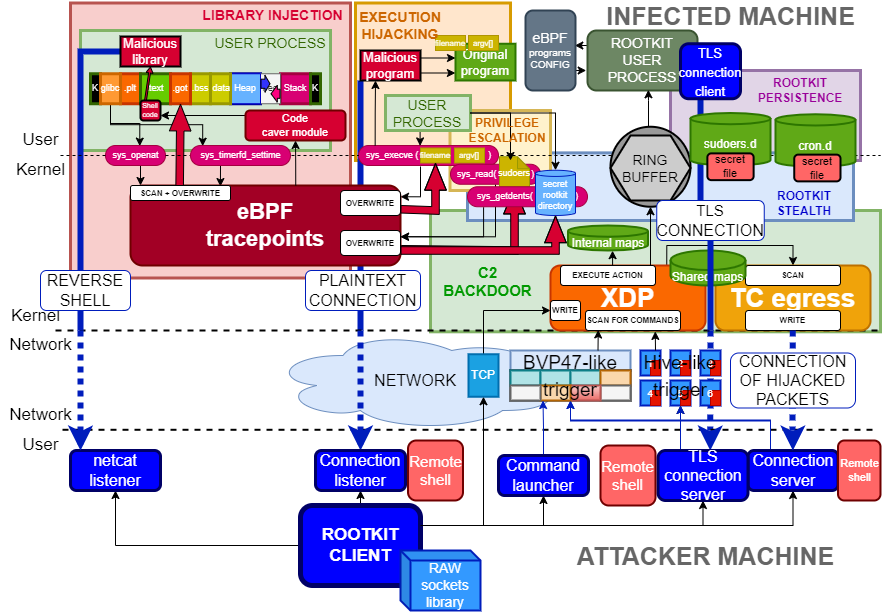
\includegraphics[width=15.5cm]{rootkit.png}
	\caption{Overview of the rootkit subsystems and components.}
	\label{fig:rootkit}
\end{figure}

As we can observe in the figure, we can distinguish 6 different rootkit modules, along with a rootkit client which provides remote control of the rootkit over the network from the attacker machine. Also, there exists a rootkit user space process, which is listening for commands issued from the kernel-side, transmitted through a ring buffer.
\begin{itemize}
\item The \textbf{user space process} of the rootkit is in charge of loading and attaching the eBPF rootkit in the kernel, and creating the eBPF maps needed for their operations. For this, it uses the eBPF programs configurator, an internal structure that manages the eBPF modules at runtime, being able to attach or deattach them after a command to do so is received.

The user space process also listens to any data received at the ring buffer, an special map which the eBPF program at the kernel will use to communicate with the user-side, issuing commands and triggering actions from it. Between others actions, the rootkit user space process can spawn TLS clients, execute malicious programs or use the eBPF program configurator for managing the eBPF programs.

\item The \textbf{library injection} module is in charge of hijacking the execution of target processes by injecting a malicious library. For this, it uses a set of eBPF tracepoints in the kernel side, and a code caver module in the user side in charge of scanning user processes and injecting shellcode, apart from the malicious library itself, which is prepared to communicate with the attacker's remote client.

\item The \textbf{execution hijacking} module is in charge of hijacking the execution of programs right before the process is even created, modifying the kernel function arguments in such a way that the a new malicious program is called, but the original information is not lost so that the malicious program can still create the original process. Therefore, it hijacks the creation of processes by transparently injecting the creation of one additional malicious process on top of the intended one.

\item The \textbf{privilege escalation} module is in charge of ensuring that any user process spawned by the rootkit will maintain full privilege in the system. Therefore, it hijacks any call to the sudoers file (on which privileged users are listed) so that the user on which the rootkit is loaded is always treated as root. Note that we have not listed this module as one of the main project objetives mainly because it acts as a helper to other modules, such as the execution hijacking one.

\item The \textbf{backdoor} is one of the most critical modules in the rootkit. It has full control over incoming traffic with an XDP program, and outgoing traffic with a TC egress program. As we will see, both the XDP and TC programs are loaded in different eBPF programs, so they use a shared eBPF map to communicate between them.

The backdoor maintains a Command and Control (C2) system that is prepared to listen for specially-crafted network triggers which intend to be stealthy and go unnoticed by network firewalls. These triggers transmit information and commands to the XDP program at the network border, which the backdoor is in charge of interpreting and issuing the corresponding actions, either by writing data at an eBPF map in which other eBPF programs are reading, or issuing an action request via the ring buffer. On top of that, the TC program interprets the data parsed by the XDP program and shapes the outgoint traffic, being able to inject secret messages into packets. 

\item The \textbf{rootkit stealth} module is in charge of implementing measures to hide the rootkit from the infected host. For this, it hijacks certain system calls so that rootkit-related files and directories are hidden from the system.

\item The \textbf{rootkit persistence} module is in charge of ensuring that the rootkit will stay loaded even after a complete reboot of the infected system. For this, it injects secret files at the \textit{cron} system (which will launch the rootkit after a reboot) and at the sudo system (which maintains the privileged permissions of the rootkit after the reboot).

\item The \textbf{rootkit client} is a command-line interface (CLI) program that enables the attacker to remotely control the rootkit at the infected machine. For this, it incorporates multiple operation modes that launch different commands and network triggers. These network triggers, and any other packet sent to the backdoor, are customly designed TCP packets sent over a raw socket, enabling to avoid the noisy TCP 3-way handshake and to control every detail of the packet fields. Each of the messages generated by the client (and sent by the backdoor) follow a custom rootkit protocol, that defines the format of the messages and allows both the client and the backdoor to identify those packets belonging to this malicious traffic. In order to craft these packets, the rootkit client uses a raw sockets library (RawTCP\_Lib) that we have developed for this purpose \cite{rawtcp_lib}.

The RawTCP\_Lib library incorporates packets building, raw socket packet transmissions, and a sniffer for incoming packets. This sniffer is particularly relevant since the client will need to listen for responses by the rootkit backdoor and quickly detect those that follow the rootkit protocol format.

Apart from the network triggers, upon receiving a response by the backdoor the rootkit client can start pseudo-shells connections (commands can be sent to the backdoor and the backdoor executes them, but no shell process is spawned in the client), or spawn TLS servers that establish an encrypted connection with the backdoor. This connection, internally, still uses the custom rootkit protocol to act as a pseudo-shell, enabling to execute commands remotey.
\end{itemize}


With respect to how the rootkit implementation is distributed into multiple programs, we can find that, overall, there exist 4 main components, as shown in figure \ref{fig:rootkit_files}.

\begin{figure}[htbp]
	\centering
	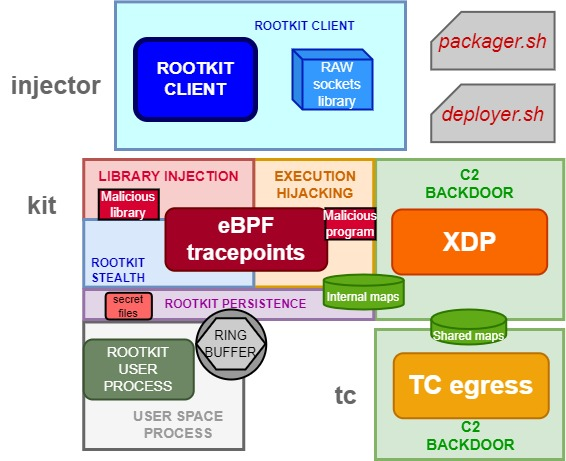
\includegraphics[width=15cm]{rootkit_files.jpg}
	\caption{Rootkit programs and scripts.}
	\label{fig:rootkit_files}
\end{figure}

As we can observe in the figure, the rootkit modules we have overviewed previously are distributed into different files:
\begin{itemize}
\item The program \textit{\textbf{injector}} comprises the rootkit client and the shared library RawTCP\_Lib. This program is to be launched from the attacker machine after a successful infection of a host.
\item The program \textit{\textbf{tc}} contains the TC program needed for managing the egress network traffic. The reason why it is loaded separately is because the libbpf library does not currently incorporate support for integrating TC programs easily as with XDP or tracepoints.

This program is also responsible of creating the shared map which the backdoor will use, and therefore it must be the first part of the rootkit loaded.
\item The program \textit{\textbf{kit}} contains most of the rootkit functionality, spawning the user process and the kernel-side eBPF programs and maps.
\item The \textit{\textbf{packager.sh}} and \textit{\textbf{deployer.sh}} files are scripts which an attacker, upon gaining access to a machine, can use to quickly set up the rootkit and infect the machine:
\begin{itemize}
	\item \textit{packager.sh} compiles the rootkit and prepares the \textit{injector}, \textit{kit} and \textit{tc} files in an output directory to be used (this directory is hidden by the rootkit once it is loaded).
	\item \textit{deployer.sh} uses the output directory to launch the rootkit files in order (first \textit{tc}, then \textit{kit}). It also injects the necessary files into the sudoers.d and cron.d directories (which will be later hidden by the rootkit) to maintain persistence.
\end{itemize}
\end{itemize}



\section{Library injection module} \label{section:lib_injection}
In this section, we will discuss how to hijack an user process running in the system so that it executes arbitrary code instructed from an eBPF program. For this, we will be injecting a library which will be executed by taking advantage of the fact that the GOT section in ELFs is flagged as writable (as we introduced in section \ref{subsection:elf_lazy_binding} and using the stack scanning technique covered in section \ref{subsection:bpf_probe_write_apps}. This injection will be stealthy (it must not crash the process), and will be able to hijack privileged programs such as systemd, so that the code is executed as root.

We will also research how to circumvent the protections which modern compilers have set in order to prevent similar attacks (when performed without eBPF), as we overview in section \ref{subsection:hardening_elf}.

This technique has some advantages and disadvantages to the one described by Jeff Dileo at DEFCON 27 \cite{evil_ebpf_p6974}, which we will briefly cover before presenting ours. Both techniques will be later compared in chapter \ref{chapter:related_work}.


\subsection{ROP with eBPF} \label{subsection:rop_ebpf}
In 2019, Jeff Dileo presented in DEFCON 27 the first technique to achieve arbitrary code execution using eBPF \cite{evil_ebpf_p6974}. For this, he used the ROP technique we described in section \ref{subsection:rop} to inject malicious code into a process. We will present an overview on his technique, in order to later compare it to the one we will develop for our rootkit, and find advantages and disadvantages. Note that this is a summary and some aspects have been simplified, however we will go in full detail during the explanation of our own technique.

Figure \ref{fig:rop_evil_ebpf_1} shows an overview on the process memory and the eBPF programs loaded. For this injection, we will use the stack scanning technique (section \ref{subsection:bpf_probe_write_apps}) using the arguments of a system call whose arguments are passed using the stack (sys\_timerfd\_settime, which receives two structs utmr and otmr). Therefore, a kprobe is attached to the system call, so that it can start to scan for the return address of the system call, which we know is the original value of register rip which was pushed into the stack (ret).

%TODO This figure needs a remodel. I tried to keep it simple to explain the main concepts on the technique described afterwards, but after writing the next section I realised it gets some things wrong:
% - It does not show .got and .plt sections.
% - It shows the RBP register in an incorrect place.
\begin{figure}[htbp]
	\centering
	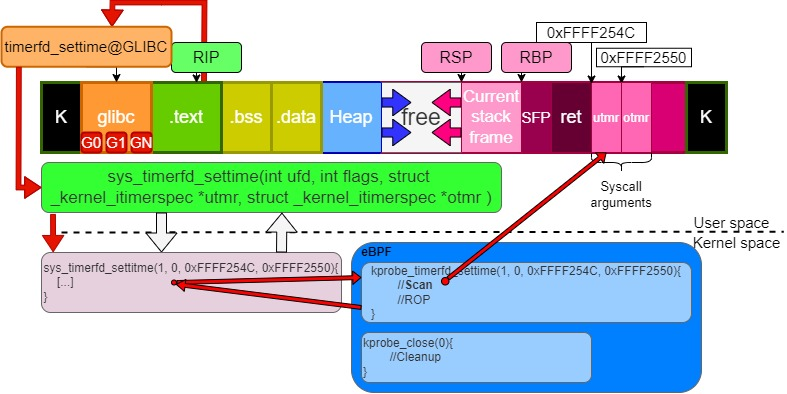
\includegraphics[width=15cm]{rop_evil_ebpf_1.jpg}
	\caption{Initial setup for the ROP with eBPF technique.}
	\label{fig:rop_evil_ebpf_1}
\end{figure}

%TODO I don't quite like this. Maybe the glibc bit, because of its importance, is better somewhere else
An additional aspect must be introduced now (we will cover it more in detail in section \ref{TODO}): system calls are not directly called by the instructions in the .text section, but rather user programs in C make use of the C Standard Library to delegate the actual syscall, which in this case is the GNU Standard Library (glibc) \cite{glibc}. Therefore, a program calls a function in glibc (in this case timerfd\_settime) in which the syscall is performed, and the kernel executes it.

This means that, during the stack scanning technique, if we start from struct utmr and scan forward in the stack, what we will find in ret is the return address of the PLT stub that calls the function at glibc, and not directly that of the syscall to the kernel. Therefore, our goal is, for every data in the stack while scanning forward, check whether it is the real return address of the PLT stub we are looking for. For an address to be the real return address, we will follow the next steps:
\begin{enumerate}
\item Take an address from the stack. If that is the return address (the saved rip), then the instruction that called the PLT stub that jumps to the function in glibc must be the previous instruction (rip - 1).
\item We now have a \textit{call} instruction, that directs us to the PLT stub. We take the address stored at the GOT section and jump to the function at glibc.
\item We scan forward, inside timerfd\_settime of glibc, until we find a \textit{syscall} instruction. That is the point where the flow of execution moves to the kernel, so we have checked that the return address we found in the stack truly is the one we are looking for.
\end{enumerate}

Now that we have found the return address, we save a backup of the stack (to recover the original data later) and we proceed to overwrite the stack using bpf\_probe\_write\_user(), setting it for the ROP technique. For this, some gadgets (G0, G1 ... GN) have been previously discovered in the glibc library. Figure \ref{fig:rop_evil_ebpf_2} shows process memory after this overwrite:

\begin{figure}[H]
	\centering
	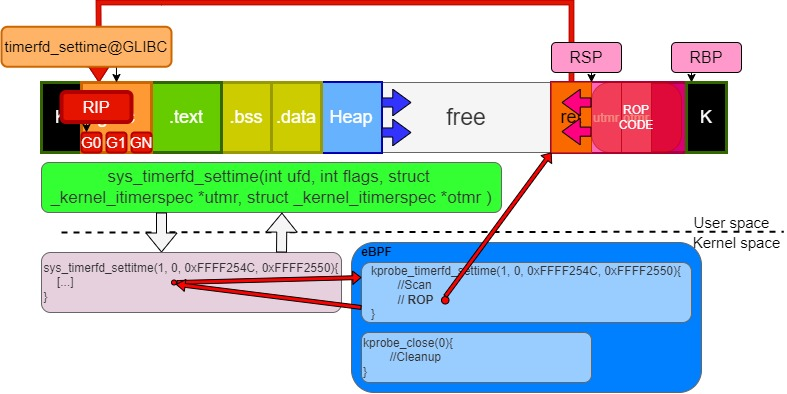
\includegraphics[width=15cm]{rop_evil_ebpf_2.jpg}
	\caption{Process memory after syscall exits and ROP code overwrites the stack.}
	\label{fig:rop_evil_ebpf_2}
\end{figure}

As we can see in the figure, the function has already exited, and ret has been popped into register rip. As we explained in section \ref{subsection:rop}, the attacker places in that position the address of the first ROP gadget. After that, the attacker can execute arbitrary code. Jeff Dileo, for instance, loads a malicious library into the process (we will do the same and explain this process in the next sections).

Once the attacker has finished executing the injected code, the stack must be restored to the original position so that the program can continue without crashing. A simplified view of this procedure consists of attaching a kprobe to a random system call (in this case, sys\_close()) so that, from the ROP code, we can alert the eBPF program when it is time to remove the ROP code and restore the original stack. Figure \ref{fig:rop_evil_ebpf_3} shows this final step:

\begin{figure}[H]
	\centering
	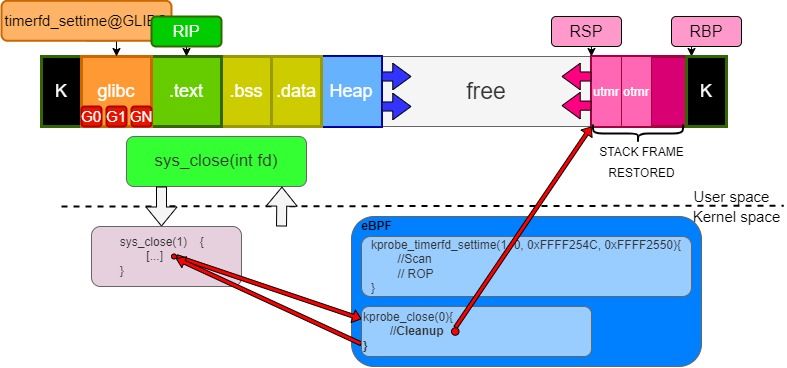
\includegraphics[width=15cm]{rop_evil_ebpf_3.jpg}
	\caption{Stack data is restored and program continues its execution.}
	\label{fig:rop_evil_ebpf_3}
\end{figure}

As we can see, eBPF writes back the original stack and thus the execution can continue. Note that, in practice, some final gadgets must also be executed in order to restore the state of rip and rsp, the stack data for this is written in the free memory zone, so that it does not need to be removed.


%TODO Eligible to writing more. This was merged with the explanation of each feature before, so it was more extense, but now it might need some more info??
\subsection{Bypassing hardening features in ELFs} \label{subsection:hardening_bypass}
During section \ref{subsection:hardening_elf}, we presented multiple  security hardening measures that have been introduced to prevent common exploitation techniques (such as stack buffer overflows) and that nowadays can be incorporated, usually by default, in ELF binaries generated using modern compilers. We will now explore how to bypass these features, so that we can design an injection technique that can target any process in the system, independently on whether it was compiled using these mitigations.

\textbf{Stack canaries}\\
Since stack canaries will be checked after the vulnerable function returns, an attacker seeking to overwrite the stack must ensure that the value of the canary remains constant. In the context of a buffer overflow attack, this can be achieved by leaking the value of the canary and incorporating it into the overflowing data at the stack, so that the same value is written on the same address \cite{canary_exploit}.

In our rootkit, unlike in the ROP technique presented in section \ref{subsection:rop_ebpf}, we will avoid overwriting the value of the saved rip in the stack completely. Therefore, as long as our eBPF program leaves all registers and stack data in the same state as before calling the function, we will not trigger any alerts.

\textbf{DEP/NX}\\
The only alternative for an attacker upon a non-executable stack is either injecting shellcode at any other executable memory address, or the use of advanced techniques like ROP that fully circumvent this mitigation since the data at the stack is not directly executed at any step.

In our rootkit, we will choose the first option, scanning the process virtual memory for an executable page where we will inject our shellcode. This process is usually known as finding 'code caves'.

\textbf{ASLR}\\
In order to bypass ASLR, attackers must take into account that, although the address at which, for instance, a library is loaded is random, the internal structure of the library remains unchanged, with all symbols in the same relative position, as figure \ref{table:aslr_offset} shows.

%TODO Add the .data section here
\begin{figure}[htbp]
	\centering
	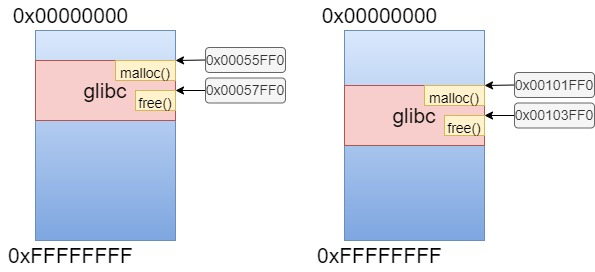
\includegraphics[width=13cm]{aslr_offset.jpg}
	\caption{Two runs of the same executable using ASLR, showing a library and two symbols.}
	\label{fig:alsr_offset}
\end{figure}

As we can observe in the figure, although glibc is loaded at a different base address each run, the offset between the functions it implements, malloc() and free(), remains constant. Therefore, a method for bypassing ASLR is to gather information about the absolute address of any symbol, which can then easily lead to knowing the address of any other if the attacker decompiles the executable and calculates the offset between a pair of addresses where one is known. This is the chosen method for our technique.

\textbf{PIE}\\
Similarly to ASLR, although the starting base address of each memory section is random, the internal structure of each section remains the same. Therefore, if an attacker is able to leak the address of some symbol in a section, and by knowing the offset at which it is located with respect to the base address of the section, then the address of any other symbol in the same section can be calculated \cite{pie_exploit}. This is the technique we will incorporate in our rootkit.

\textbf{RELRO}\\
If an executable was compiled using Partial RELRO, then the value of GOT can still be overwritten. If in turn it was compiled using Full RELRO, this stops any attempt of GOT hijacking, unless an attacker finds an alternative method for writing into the virtual memory of a process that bypasses the read-only flag. 

In our rootkit, we will directly write using eBPF the value of GOT if it was compiled with Partial RELRO, and use an alternative technique for writing into the virtual memory of a process whenever it was compiled using Full RELRO.


\subsection{Library injection via GOT hijacking} \label{subsection:got_attack}
Taking into account the previous background and that about stack attacks, ELF's lazy binding and hardening features for binaries we presented in section \ref{section:elf}, we will now present the exploitation technique incorporated in our rootkit to inject a malicious library into a running process. 

This attack is based on the possibility of overwriting the data at the GOT section. As we have mentioned previously, this section is marked as writeable if the program was compiled using Partial RELRO, meaning that we will be able to overwrite its value from an eBPF program using the helper bpf\_probe\_write\_user(). After modifying the value of GOT, a PLT stub will take the new value as the jump address (as we explained in section \ref{subsection:elf_lazy_binding}), effectively hijacking the flow of execution of the program. In the case that a program was compiled with Full RELRO (which will be the case of many programs running by default in a Linux system such as systemd), we will make use of the /proc filesystem for overwriting this value.

The rootkit will inject the library once an specific syscall is called by a process, but the library injection will only happen after the second syscall, since we need to wait for the GOT address to be loaded by the dynamic linker. This is a necessary step because eBPF will need to validate that it really is the GOT section to overwrite.

This technique works both in compilers with low hardening fetaures by default (Clang) and also on a compiler with all of them active (GCC), see table \ref{table:compilers}. On each of the steps, we will detail the different existing methods depending on the compiler features.

For this research work, the rootkit is prepared to perform this attack on any process that makes use of either the system call sys\_openat or sys\_timerfd\_settime, which are called by the standard library glibc.

We will now describe the multiple exploitation stages for our technique. Figure \ref{fig:flow_lib_injection_compact} shows a flow diagram with the complete process.

\begin{figure}[htbp]
	\centering
	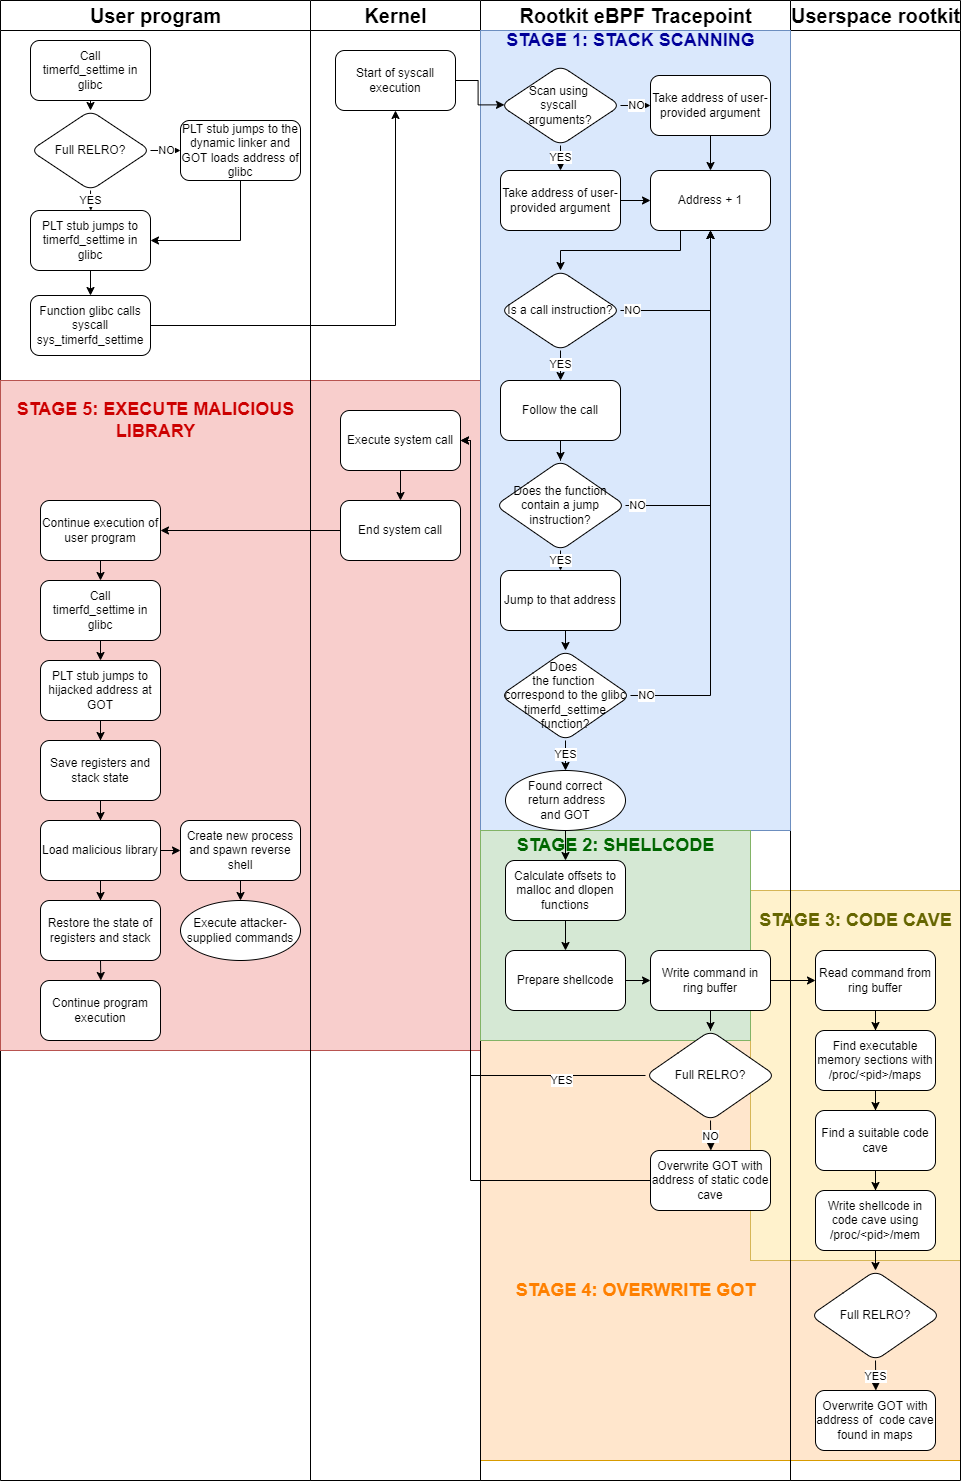
\includegraphics[width=15cm]{flow_lib_injection_compact.png}
	\caption{Flow diagram of execution of a successful library injection.}
	\label{fig:flow_lib_injection_compact}
\end{figure}

\textbf{Stage 1: eBPF tracing and scan the stack}\\
We load and attach a tracepoint eBPF program at the \textit{enter} position of syscall sys\_timerfd\_settime. Firstly, we must ensure that the process calling the tracepoint is one of the processes to hijack.

We will then proceed with the stack scanning technique, as we explained in section \ref{subsection:bpf_probe_write_apps}. In this case, we will take one of the syscall parameters and scan forward in the stack. For each iteration, we must check if the data at the stack corresponds to the saved return address of the PLT stub that jumps to glibc where the syscall sys\_timerfd\_settime is called. Figure \ref{fig:lib_stage1} shows an overview of how these call instructions relate each memory section. 


\begin{figure}[htbp]
	\centering
	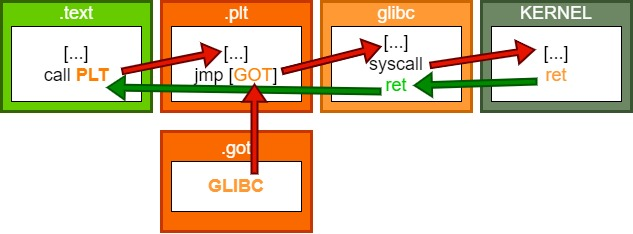
\includegraphics[width=13cm]{plt_got_glibc_flow.jpg}
	\caption{Overview of jump and return instructions from the program instructions to the syscall at the kernel.}
	\label{fig:lib_stage1}
\end{figure}

The following are the steps we will follow to perform check some data at the stack is the saved return address:
\begin{enumerate}
\item Check that the previous instruction is a call instruction, by checking the instruction length and opcodes (call instructions always start with e8, and the length is 5 bytes, see figure \ref{fig:firstcall}).
\begin{figure}[htbp]
	\centering
	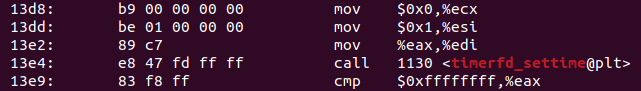
\includegraphics[width=13cm]{sch_firstcall.png}
	\caption{Call to the glibc function, using objdump.}
	\label{fig:firstcall}
\end{figure}
\item Now that we know we localized a call instruction, we take the address at which it jumps. That should be an address in a PLT stub.
\item We analyse the instructions at the PLT stub. If the program was compiled with GCC, the first instruction will be an \textit{endbr64} instruction followed by the PLT jump instruction using the address at GOT (see figure \ref{fig:plt_gcc}), since it generates Intel CET-compatible programs. Otherwise, if using Clang, which does not generate Intel CET instructions, the first instruction is the PLT jump (see figure \ref{fig:plt_clang}).

We analyse the jump instruction and, again, take the address at which it jumps. This time, it should be the address of the function at glibc.
\begin{figure}[htbp]
	\centering
	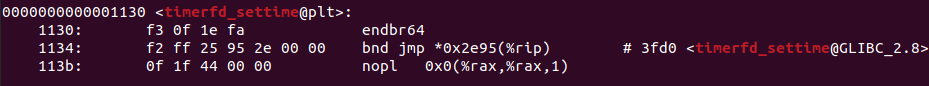
\includegraphics[width=14cm]{sch_plt_gcc.png}
	\caption{PLT stub generated with gcc compiler, using objdump.}
	\label{fig:plt_gcc}
\end{figure}
\begin{figure}[htbp]
	\centering
	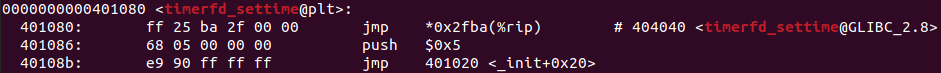
\includegraphics[width=14cm]{sch_plt_clang.png}
	\caption{PLT stub generated with clang compiler, using objdump.}
	\label{fig:plt_clang}
\end{figure}

\item We now have the address of timerfd\_settime at glibc, from where the syscall will be called. From eBPF, we continue to scan the first opcodes and compare them to those we expect to find at glibc. Specifically, the function would have to contain the instruction opcodes shown in figure \ref{fig:settime_glibc}. Note that, in our version of Ubuntu, we will find Glibc compiled with GCC.

\begin{figure}[htbp]
	\centering
	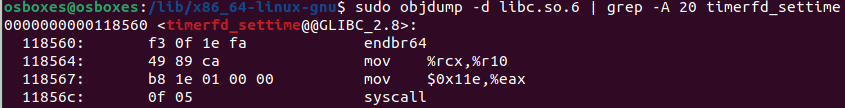
\includegraphics[width=14cm]{sch_settime_glibc.png}
	\caption{Timerfd\_settime function at glibc, using objdump.}
	\label{fig:settime_glibc}
\end{figure}

\end{enumerate}

Once we ensured we reached the correct glibc function, we are now sure that the data we found at the stack is the return address of the PLT stub that jumped to glibc and called the syscall sys\_timerfd\_settime. Most importantly, we know the address of the GOT section which we want to overwrite.

Our rootkit also incorporates an alternative scanning technique for processes calling the syscall sys\_openat(). This technique enables to scan the stack even when the system call does not incorporate any arguments from the userspace (and thus we cannot take them from our eBPF tracing program to use them as a foothold in the stack).

As we explained in section \ref{subsection:tracing_arguments}, tracepoint programs receive an struct pt\_regs pointer as an argument. We can take this struct and use the value of register rbp as our starting point for scanning the stack. As we can see on figures \ref{fig:plt_clang}, \ref{fig:plt_gcc} and \ref{fig:settime_glibc}, the  PLT does not contain any function prologue (it does not modify the value of rsp) and the function at glibc does not change this value either. Therefore, in our eBPF program, since we are hooking the syscall at the beginning of its execution, the value of rbp will be the original frame pointer before calling the PLT, and therefore we can use it as our starting address for stack scan, proceeding to scan forward until we find the saved return address.

\textbf{Stage 2: Programming shellcode}\\
Once that we have the address of the GOT section, we need to prepare our shellcode to be injected into the process memory. We will overwrite the value at GOT and redirect the flow of execution to the address at which our shellcode is stored in memory. 

Since we want our shellcode to be able to load a library, it will need to call the function \_\_libc\_dlopen\_mode, which can be found in glibc. This function expects to receive as an argument a string with the file path of the malicious library, and therefore the shellcode will also need to call \_\_libc\_malloc to allocate space for the argument. Tables \ref{table:libc_malloc} and \ref{table:libc_dlopen_mode} explain the expected arguments and return value of each function in detail.

\begin{table}[htbp]
\begin{tabular}{|>{\centering\arraybackslash}p{4cm}|>{\centering\arraybackslash}p{10cm}|}
\hline
Register & Value\\
\hline
\hline
edi & Number of bytes to allocate. \\
\hline
rax & Return value, contains the address at which the requested bytes were allocated\\
\hline
\end{tabular}
\caption{Arguments and return value of function \_\_libc\_malloc.}
\label{table:libc_malloc}
\end{table}

\begin{table}[htbp]
\begin{tabular}{|>{\centering\arraybackslash}p{4cm}|>{\centering\arraybackslash}p{10cm}|}
\hline
Register & Value\\
\hline
\hline
rsi & 0x1, indicating flag RTLD\_LAZY\\
\hline
rdi & Address where to read path of library to load\\
\hline
\end{tabular}
\caption{Arguments of function \_\_libc\_dlopen\_mode.}
\label{table:libc_dlopen_mode}
\end{table}

The programs were compiled having ASLR active, and therefore we cannot know the virtual address at which these functions are loaded into the process memory. However, since we have leaked the address of timerfd\_settime at glibc with the previous eBPF scan, we can calculate the address of the other functions, as we introduced in section \ref{subsection:hardening_bypass}. Figure \ref{fig:aslr_bypass_example} shows an example of this process.

\begin{figure}[htbp]
	\centering
	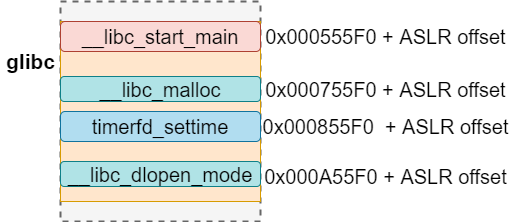
\includegraphics[width=10cm]{aslr_bypass_example.png}
	\caption{Functions at glibc with ASLR active.}
	\label{fig:aslr_bypass_example}
\end{figure}

We will use the example of the figure to illustrate how to calculate the address of the functions:
\begin{enumerate}
\item Decompile using objdump the glibc diagram and calculate the constant offset between the timerfd\_settime function (whose address we will know at runtime) and a reference function usually found in the first addresses of glibc, in this case \_\_libc\_start\_main (this step can be avoided, but it is recommended when searching for many functions and to avoid working with negative offsets). In the example, this offset is 0x30000.
\item Calculate the offset from the reference function \_\_libc\_start\_main to \_\_libc\_dlopen\_mode and \_\_libc\_malloc. In the example, this is 0x20000 and 0x5000 respectively by looking at  decompiled glibc.
\item During runtime, although the ASLR offset will be applied, it will skew all functions inside glibc by the same amount, and therefore the offsets previously calculated will be maintained. By using the previously, calculated offsets, we get that:
\begin{itemize}
	\item \_\_libc\_start\_main = timerfd\_settime - 0x30000
	\item \_\_libc\_dlopen\_mode = \_\_libc\_start\_main + 0x50000
	\item \_\_libc\_malloc = \_\_libc\_start\_main + 0x20000
\end{itemize}
\end{enumerate}

Once we know the address of the functions we want our shellcode to call, we can start to develop it. We will program an x86\_64 assembly program, from which we will extract its opcodes. The shellcode will follow the next algorithm:
\begin{enumerate}
\item Backup the value of all registers, including rbp and rsp. We must ensure that the stack frame is not modified after the shellcode ends, otherwise we may trigger a stack canary alert.
\item Allocate memory for the pathname of the library at the heap using \_\_libc\_malloc.
\item Write into the allocated memory the pathname of our library to load.
\item Call \_\_libc\_dlopen\_mode indicating the allocated memory with the library pathname. Before doing this, we found that reserving an additional stack frame reduces the chances of the process crashing, since apparently the function modifies the stack. By moving rbp and rsp, we prevent the function from modifying any pre-existing data.
\item Restore the original value of the registers, and jump back to the original system call which the glibc function intended to call.
\end{enumerate}

The complete developed shellcode and its opcodes can be found in Appendix \ref{annex:shellcode}.


\textbf{Stage 3: Injecting shellcode in a code cave}\\
Once we have developed our shellcode, and before overwriting the value of GOT, we need to find a memory section where to write our shellcode, so that we can executing the necessary instructions to inject our malicious library. This area must be large enough to fit our shellcode, and it must be marked as executable. 

Because of DEP/NX, we cannot use the stack for executing code. On top of that, as we can observe in the section header dump at Appendix \ref{annexsec:readelf_sec_headers}, for security reasons all sections are nowadays marked either writeable or executable, but never both simultaneously.

Therefore, we will use the proc filesystem which we introduced in section \ref{section:proc_filesystem}. By using the file under \textit{/proc/<pid>/maps}, we will easily identify the address range of those memory sections marked as executable, and by using the file \textit{/proc/<pid>/mem}, we will write our shellcode into that memory section, bypassing the absence of a write flag.

Although we may write freely into any virtual address using this technique, as we saw in section \ref{subsection:proc_maps} executable memory usually corresponds to the .text section. Therefore, we are at risk of overwriting critical instructions of the program. This is the reason why we must search for empty memory spaces inside the virtual memory, called code caves.

We will consider an appropiate code cave as a continuous memory space inside the .text section that consists of a series of NULL bytes (opcode 0x00). Although in principle this may seem like a rare occurence, it is a common find in most processes due to how memory access control is implemented.

In figure \ref{fig:proc_maps_sample}, we can observe how virtual memory sections have a length of 0x1000, or are a multiple of it. This is not an arbitrary number, but rather it is because memory sections must always be of length multiple of the system page length (4 KB = 0x1000 bytes). Therefore, the minimum granularity of a set of permissions over a memory section is of 0x1000 bytes.

Since sections must occupy a multiple of 1000 bytes, this leads to multiple sections which leave lots of empty, NULL bytes, unocuppied without any instructions. This is the reason why we will, quite probably, find a code cave in most processes.

Therefore the steps to find a code cave and inject our shellcode are the following:
\begin{itemize}
\item Send a command from eBPF to the rootkit user space program, indicating that we want to find a code cave in process with an specific PID.
\item Iterate over each entry of \textit{/proc/<pid>/maps}, looking for a sufficiently large code cave in an executable memory section.
\item Inject the shellcode into the code cave using \textit{/proc/<pid>/mem}.
\end{itemize}

Note that, although we used the \textit{/proc/<pid>/maps} file for finding a code cave, this can still be done using the helper bpf\_probe\_read (by taking the return address at the stack and scanning forward in the .text section) or, in the case of programs compiled without PIE, finding an static code cave at the .text section by decompiling the program (since the .text section will be loaded at the same position on every program execution). Still, we would have needed to use \textit{/proc/<pid>/mem} for bypassing the write access prevention.

\textbf{Stage 4: Overwriting GOT}\\
Once the shellcode is loaded at the code cave, eBPF can proceed to overwrite the GOT value with the address of the code cave. As we mentioned, this address is writable using the helper bpf\_probe\_write\_user() if the program was compiled using Partial RELRO, but it cannot be modified if Full RELRO was used. 

Therefore, our rootkit will modify GOT using bpf\_probe\_write\_user() with the address of an static code cave for those programs compiled with Clang (Partial RELRO, no PIE), and use \textit{/proc/<pid>/mem} for modifying GOT with the value of code cave found using \textit{/proc/<pid>/maps} for those programs compiled using GCC (Full RELRO, PIE active).

\textbf{Stage 5: Second syscall, execution of the library}\\
Once we have overwriten GOT with the address of our code cave, the next time the same syscall is called, the PLT stub will jump to our code cave and execute our shellcode. As instructed by it, the malicious library will be loaded and afterwards the flow of execution jumps back to the original glibc function.

%Explain reverse shell?
With respect to the malicious library, it forks the process (to keep the malicious execution in the background) and spawns a simple reverse shell which the attacker can use to execute remote commands.


\section{Privilege escalation module} \label{subsection:privesc}
In this section we will discuss how the rootkit tampers with the access control permissions in the system, so that unprivileged programs gain root access. Although it is based on a simple technique, it will be used to support other modules launching malicious programs with full privilege (such as the execution hijacking module).

Therefore, the purpose of this section is that, without having to introduce any password, programs executed by an unprivileged user can enjoy privileged access in a infected system.

\subsection{Sudoers file}
Sometimes, unprivileged users need to run a program requiring privileged access. For this, Linux systems incorporate the sudo security policy module, which sets a 'sudo' privilege on users and user groups, allowing them to run a program as root. 

The most widespread and default sudo security policy module is the 'sudoers' policy module, which sets the available sudo permissions of users and groups in the \textit{/etc/sudoers} file \cite{sudoers_man}. In this file, the system administrator can determine the specific permissions of each entity and set different options, including whether they need to introduce the user password when using the 'sudo' command, which is particularly relevant for us. Figure \ref{fig:sudoers} shows the \textit{/etc/sudoers} file of the host we will infect with our rootkit.

\begin{figure}[htbp]
	\centering
	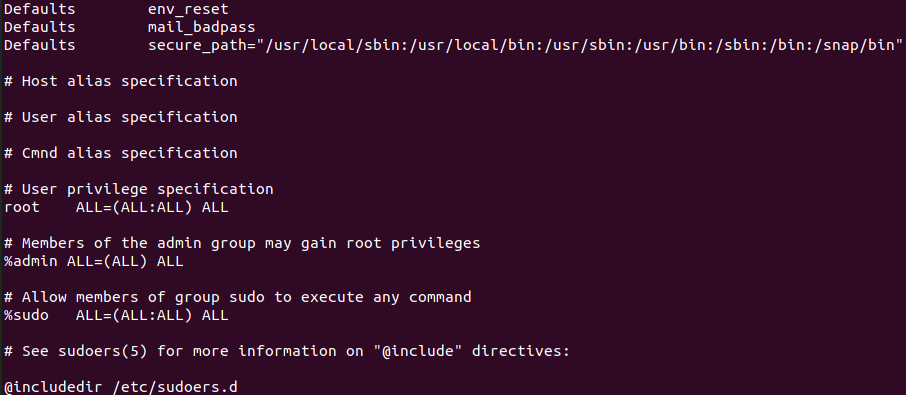
\includegraphics[width=10cm]{sch_sudoers.png}
	\caption{/etc/sudoers file of infected host.}
	\label{fig:sudoers}
\end{figure}

As we can observe in the figure, members of the sudo group are allowed to execute any command as root. Figure \ref{fig:groupfile} shows the users which belong to this group.

\begin{figure}[htbp]
	\centering
	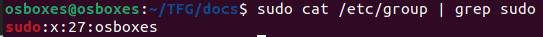
\includegraphics[width=10cm]{sch_groupfile.png}
	\caption{/etc/group file in the infected host.}
	\label{fig:groupfile}
\end{figure}

As we can appreciate, the user osboxes (the default user in the host) is included in this group, and therefore this user is allowed to use sudo and run commands as root.

Any user can check its current sudo privileges by running the command \lstinline{sudo -l} \lstinline{}. Figure \ref{fig:sudol} shows this for the osboxes user.

\begin{figure}[htbp]
	\centering
	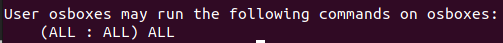
\includegraphics[width=10cm]{sch_sudol.png}
	\caption{Sudo privileges of user osboxes, with sudo -l.}
	\label{fig:sudol}
\end{figure}

The value of these entries is taken from the parameters set in figure \ref{fig:sudoers}, where each of the ALL values mean:
\begin{itemize}
\item First ALL: Any user of the group
\item Second ALL: Any host
\item Third ALL: As any user
\item Fourth ALL: Any command
\end{itemize}

Therefore, user osboxes, as part of the sudo group, may run any command as any user in any host as sudo. The host part is not relevant for our us, since it is used when a single sudoers file is distributed betweem multiple machines, but we still have to follow the appropiate format when writing an entry in the \textit{/etc/sudoers} file.

Each time we execute a command with sudo, a process named 'sudo' will open and read the \textit{/etc/sudoers} file, interpreting the contents and allowing or rejecting the action. Note that, although once an user introduces the sudo password it may not be asked again for a period of time, the sudo process will still open and read the \textit{/etc/sudoers} file for each time sudo is used. This aspect is particularly relevant for our technique.


\subsection{Hijacking sudoers read accesses}
We will now discuss how our rootkit tampers with the sudoers policy module. The technique we will present is based on modifying the content that the sudo process reads from the \textit{/etc/sudoers} file, so that what the user process receives is different than that contained in the file. By crafting some special entries in the file, we can grant automatic password-less access to any process we want.

In order to read the contents from the \textit{/etc/sudoers} file, the sudo process will need to perform the following actions:
\begin{itemize}
\item Open the file, using the syscall sys\_openat.
\item Read the file, using the syscall sys\_read.
\end{itemize}

Note that some intermediate or additional syscalls such as sys\_newfstatat, sys\_lseek or sys\_close are also called, but we are not considering them for simplicity.

Table \ref{table:sudoers_syscall} shows the parameters expected by these system calls, based on \cite{syscall_reference}.

\begin{table}[htbp]
\begin{tabular}{|c|>{\centering\arraybackslash}p{8cm}|}
\hline
System call & Arguments\\
\hline
\hline
\multirow{4}{*}{sys\_openat} & \multicolumn{1}{c|}{int dfd}\\
\cline{2-2}
& \multicolumn{1}{c|}{const char \_\_user *filename}\\
\cline{2-2}
& \multicolumn{1}{c|}{inf flags} \\
\cline{2-2}
& \multicolumn{1}{c|}{umode\_t umode} \\
\hline
\multirow{3}{*}{sys\_read} & \multicolumn{1}{c|}{unsigned int fd}\\
\cline{2-2}
& \multicolumn{1}{c|}{char \_\_user *buf} \\
\cline{2-2}
& \multicolumn{1}{c|}{size\_t count} \\
\hline
\end{tabular}
\caption{Arguments of syscalls used by sudo process.}
\label{table:sudoers_syscall}
\end{table}

The table shows that there exist two arguments marked as \textit{\_\_user}, which, as we explained in section \ref{subsection:bpf_probe_write_apps}, can be overwritten from an eBPF tracing program using the helper bpf\_probe\_write\_user(). Therefore, there exist two different attack vectors:
\begin{itemize}
\item Modify the argument \textit{filename}, so that the sudo process opens a fake, crafted sudoers file. In this file we would write the entries needed for our user to have sudo privilege without a password. Since the sys\_open syscall returns a file descriptor, which is later used by sys\_read, that is the only argument needed to be modified.
\item Modify the buffer \textit{buf} in the sys\_read syscall so that it returns specially crafted data to the sudo program.
\end{itemize}

Although the first option is easier, the second technique can not only apply to reading files, but also to any system calls that loads data into an user buffer. Therefore, the privilege escalation module will incorporate the second technique to show the potential of eBPF in this area.

Figure \ref{fig:privilege_esc_module} shows the complete process of the technique we will use.
\begin{figure}[htbp]
	\centering
	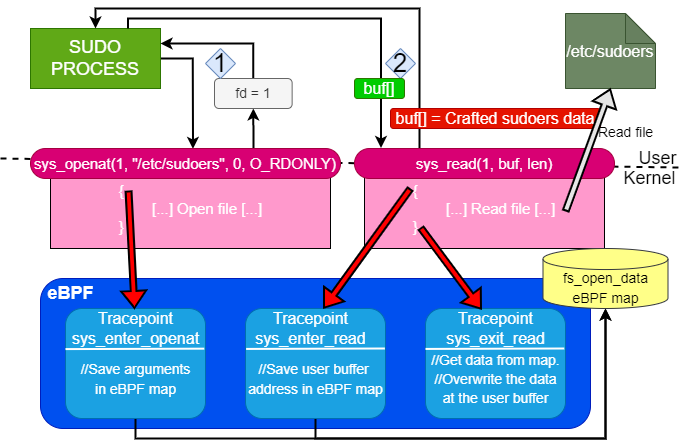
\includegraphics[width=15cm]{privilege_esc_module.png}
	\caption{Buffer overwrite technique for the privilege escalation module.}
	\label{fig:privilege_esc_module}
\end{figure}

As we can observe in the figure, we will use three eBPF tracepoints. The reason for this is that, although we are able to write into the user buffer at any tracepoint attached to sys\_read, we would lack information with only one tracepoint:
\begin{itemize}
\item An \textit{enter} tracepoint at sys\_openat knows the file being opened, but it does not have access to the user buffer.
\item An \textit{enter} tracepoint at sys\_read has access to the user buffer, but does not know the name of the file (it only has a file descriptor). Also, if it writes into the buffer now, it will be overwritten later when the kernel reads the \textit{/etc/sudoers} file.
\item An \textit{exit} tracepoint at sys\_read only receives the return value as a parameter (as we explained in section \ref{subsection:tracing_arguments}), but it can freely write to the user buffer if it had access to it, since the kernel already finished writing on it.
\end{itemize}

Taking the above into account, we designed the privilege escalation technique as follows:
\begin{enumerate}
\item We load and attach three eBPF tracepoint programs, and an eBPF map:
\begin{itemize}
	\item An \textit{enter} tracepoint attached to sys\_openat (sys\_enter\_openat).
	\item An \textit{enter} tracepoint attached to sys\_read (sys\_enter\_read).
	\item An \textit{exit} tracepoint attached to sys\_read (sys\_exit\_read).
	\item An eBPF map (fs\_open) that stores fs\_open\_data structs, composed of:
	\begin{itemize}
	\item A process name.
	\item A filename.
	\end{itemize}
	The key of the map fs\_open is the PID of the user process from which the call to an eBPF program originated, this can be obtained using the bpf\_get\_current\_pid\_tgid() helper (see section \ref{subsection:ebpf_helpers}).
\end{itemize}
\item A malicious program we executed from user "osboxes" requests sudo privileges. Our goal is to let it run with privileged permissions without having to introduce a password. Note that, although in the system we are using osboxes is an user in the \textit{/etc/sudoers} file already (although requiring a password for running as sudo), this process also works if we used an user not included on it in the first place.

The sudo process opens the \textit{/etc/sudoers} file. The syscall is called and the sys\_enter\_openat tracepoint is called before the syscall is executed. We check that the syscall was called by the sudo process using the helper bpf\_get\_current\_comm() (see section \ref{subsection:ebpf_helpers}) and, if it is, write the filename into the fs\_open map. After that, the tracepoint exists and the syscall is executed.

\item The sudo process now reads from the file descriptor of the file \textit{/etc/sudoers}. The sys\_enter\_read tracepoint is executed right before the syscall is called. In the tracepoint, we check if we can find an entry with a filename in the fs\_open map using the process PID as key (which is the same for all tracepoints, since they originated from the same sudo process). We now write address of the buffer supplied by the sudo process into the map.

\item The sys\_read syscall is executed and, when it is about to exit, our tracepoint sys\_exit\_read is executed. We take the filename and the address of the user buffer from the fs\_open map, and overwrite the data at the user buffer which contained the bytes read from \textit{/etc/sudoers} using bpf\_probe\_write\_user(). The data we will write resembles a real entry of the \textit{/etc/sudoers} file:
\begin{verbatim}
osboxes ALL=(ALL:ALL) NOPASSWD:ALL #
\end{verbatim}

Injecting that string into the read file will grant us with password-less sudo privileges. There are two particularly relevant details on it:
\begin{itemize}
\item The NOPASSWD option instructs sudo not to request a password.
\item A \# symbol is included at the end so that any data not overwritten at that line is considered a comment (see figure \ref{fig:sudoers}).
\end{itemize}

Although the previous is sufficient for tricking the sudo process into believing we have sudo privileges, it can happen that an user (in this case, osboxes) already has an entry in the \textit{/etc/sudoers} file. When this happens, the sudo process usually chooses the last entry that appears on the file or fails. 

Although not the most elegant solution, the solution for this issue incorporated in our rootkit is that the tracepoint program will continue writing \# symbols until an error happens (thus indicating we reached the end of the file).

\end{enumerate}


\section{Execution hijacking module} \label{section:execution_hijack}
This section describes how the rootkit can hijack the execution of programs. Although in principle eBPF in the kernel cannot start the execution of a program by itself, this module shows how a malicious rootkit may take advantage of benign programs in order to execute malicious code in the user space. Therefore, we aim to achieve two main goals:
\begin{itemize}
\item Execute a malicious user program taking advantage of other program's execution.
\item Be transparent to the user space, that is, if we hijack the execution of a program so that another is run, the original program should be executed too with the least delay.
\end{itemize}

This technique is based on the modification of the arguments of the system call sys\_execve, used to execute programs. When it is called, it causes the program that is currently being run to be completely replaced by the new executed program \cite{execve_man}. Its arguments are listed in table \ref{table:execve_args}

\begin{table}[htbp]
\begin{tabular}{|c|>{\centering\arraybackslash}p{7cm}|}
\hline
Argument & Description\\
\hline
\hline
const char \_\_user *filename & Path and filename of the file to execute\\
\hline
const char \_\_user *const \_\_user *argv & NULL-terminated array with arguments passed to the program\\
\hline
const char \_\_user *const \_\_user *envp & NULL-terminated array with the environment variables associated to the executed program \cite{environ}\\
\hline
\end{tabular}
\caption{Arguments of system call sys\_execve.}
\label{table:execve_args}
\end{table}

As we can observe in the table, all of the arguments of the syscall are marked with the keyword \_\_user, and therefore as we explain in section \ref{subsection:bpf_probe_write_apps} these arguments can be overwritten using the eBPF helper bpf\_probe\_write\_user(). This opens for us the possibility of modifying these arguments so that another file is modified.

Figure \ref{fig:summ_execve_hijack} summarizes the results of an attack using this rootkit module. As we can observe in the figure, we will hijack the execution of sys\_execve to run our own program, but as we mentioned we must execute the original program too in order not to raise concerns in the user space. Therefore, the malicious program must be able to access the original arguments of the sys\_execve call to execute the original program.

\begin{figure}[htbp]
	\centering
	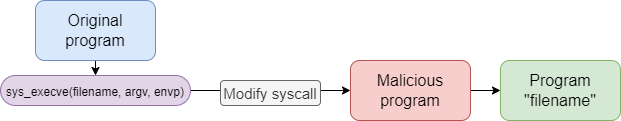
\includegraphics[width=14cm]{summ_execve_hijack.png}
	\caption{Overview of execution hijacking attack.}
	\label{fig:summ_execve_hijack}
\end{figure}

As we will discuss, apart from running the original program, the malicious program will run itself as sudo (taking advantage of the privilege escalation module) and then connecting to the rootkit client.


\subsection{Overwriting sys\_execve} \label{subsection:sys_execve_writing}
We have mentioned the possibility of overwriting the parameters of the sys\_execve syscall. However, after loading an eBPF \textit{enter} tracepoint attached to sys\_execve and writing into any of this buffers, we found three scenarios:
\begin{itemize}
\item The helper successfully overwrites the user buffers.
\item The helper fails to overwrite all or some of the buffers.
\item The helper successfully overwrites a buffer but, with a single write operation, it has also modified the value of some other user buffer.
\end{itemize}

The reason for this is that, as we covered in section \ref{subsection:bpf_probe_write_apps}, the bpf\_probe\_write\_user() helper fails to write any data in the occurence of a page fault. As we explained in section \ref{subsection:mem_faults}, minor memory faults are particularly common when executing a fork() of a process, since the child process will not get its page table completely copied from the parent, but will request the mapping once it is attempted to be read.

Because of the fact that programs calling sys\_execve will be completely replaced by the new program, we can find this function used commonly in two contexts:
\begin{itemize}
\item User programs which execute a new program as a child, but they do not want to be terminated themselves. For this, they call a fork() and then execute execve() (which calls the sys\_execve syscall) in the child process.
\item Programs that are run by the user in the command-line interface. Once a command is introduced, the program corresponding to the command is searched, and the bash process (or any other shell being used) will fork() itself and execute the new program.
\end{itemize}

Therefore, when modifying the arguments of sys\_execve, we will find that most calls are from programs which had executed fork() previously, thus having a high probability of failing. Note that the exact reason why writing one buffer with bpf\_probe\_write\_user() modifies multiple buffers simultaneouslly is unknown, but it is a situation we must account for, since we cannot trust in the helper not returning an error, we must check the result of this write accesses.

\subsection{Hiding data in a system call}
Apart from having to take into account that the bpf\_probe\_write\_user helper may fail in unexpected manners as we described, we also need to give special attention to how we will preserve the original information of the program being executed via sys\_execve after we modify the arguments of this call. As we showed in figure \ref{fig:summ_execve_hijack}, the malicious program executed using the hijacked syscall must be able to execute the original program. For this, the program will fork() and create a child process, on which execve() will be called with the original program arguments. Therefore, the main issue would be how to recover the original arguments once they were overwritten by eBPF.

In order to achieve this, we will hide the original arguments in those passed to the malicious program. Table \ref{fig:execve_args_hide} shows how this process works with a sample sys\_execve call. Environment variables have been omitted for simpleness, but we can usually find a large array of them.

\begin{table}[H]
\begin{tabular}{|>{\centering\arraybackslash}p{2cm}|>{\centering\arraybackslash}p{3cm}|}
\hline
\multicolumn{2}{|c|}{Original arguments}\\
\hline
\hline
filename & "/bin/ls"\\
\hline
argv[0] & "ls"\\
\hline
argv[1] & "-l"\\
\hline
argv[2] & NULL\\
\hline
envp[0] & NULL\\
\hline
\end{tabular}
\quad
\begin{tabular}{|>{\centering\arraybackslash}p{2cm}|>{\centering\arraybackslash}p{3cm}|}
\hline
\multicolumn{2}{|c|}{Modified arguments}\\
\hline
\hline
filename & "/home/osboxes/execve\_hijack"\\
\hline
argv[0] & "/bin/ls"\\
\hline
argv[1] & "-l"\\
\hline
argv[2] & NULL\\
\hline
envp[0] & NULL\\
\hline
\end{tabular}
\caption{Hiding data in sys\_execve arguments.}
\label{table:execve_args_hide}
\end{table}

As we can observe in the table, we will modify the value of \tetxit{filename} with the malicious program filename, and save the original filename into argv[0]. Performing this substitution means losing little information since the argv[0] argument contains the name of the program \cite{c_standard_main}, information that can also be taken from the filename (thus it can be recovered later). Only in very specific use cases the argv[0] argument is different from the file included in the filename argument (like in Busybox \cite{busybox_argv}). 

After the above substitution, the malicious program (in the table, "execve\_hijack") will be called, whose main function receives the following arguments:

\begin{verbatim}
int main (int argc, char *argv[], char *envp[]){}
\end{verbatim}

Hence, the malicious program will use the argv[] and envp[] arrays to make another sys\_execve call with the original arguments, running the original program. 

\subsection{Hijacking a program execution}
Once we have analysed the two fundamental issues regarding this module (bpf\_probe\_write\_user fails and hiding information in the syscall arguments) we will now analyze the execution hijacking module in detail using a sample program execution.

Figure \ref{fig:execve_hijack_overall} shows an overview on how the eBPF program will proceed to overwrite a sys\_execve call.

\begin{figure}[htbp]
	\centering
	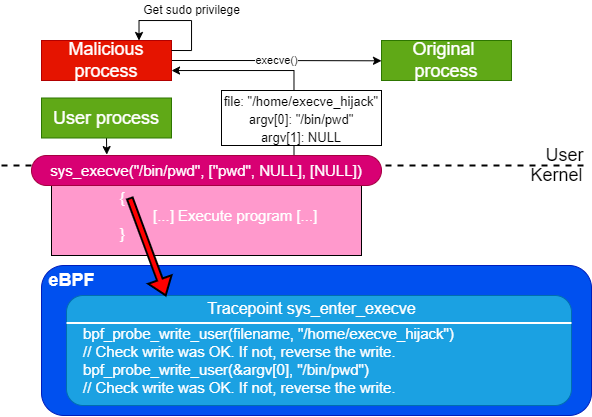
\includegraphics[width=14cm]{execve_hijack_overall.png}
	\caption{Ebpf programs used in execution hijack attack.}
	\label{fig:execve_hijack_overall}
\end{figure}

As we can observe in the figure, the steps followed will be the following:
\begin{enumerate}
\item Load and attach an eBPF \textit{enter} tracepoint attached to syscall sys\_execve (sys\_enter\_execve). 
\item When a sys\_execve is called, the eBPF program proceeds to overwrite the syscall arguments so that, instead of the intended program, the malicious program (in the figure, "execve\_hijack") is executed. For this, it will follow the next steps:

\begin{enumerate}
	\item Check using the helper bpf\_get\_current\_comm() that we are hooking the syscall of our target program. For instance, if we are targeting the commands entered by the user in the terminal, we would look for process \textit{bash}.
	\item Backup the values of the filename and all arguments.
	\item Write using bpf\_probe\_write\_user into the filename, subtituting it with the filename of our malicious program.
	\item Check that the write call was successful, and that the values of the arguments are still the same as before (since as we explained in section \ref{subsection:sys_execve_writing}, these may be modified simultaneously). If one of these errors happened, we will write back into the filename the original program filename, and exit from the tracepoint.
	\item Write using bpf\_probe\_write\_user into the first argument argv[0], subtituting it with the filename of the original program.
	\item Check again that the write call was successful, and that the values of the arguments are still the same as before. If one of these errors happened, we will write back into the argv[0] the original argument, and exit from the tracepoint.
\end{enumerate}
\item If the previous steps were executed successfully, once we exit from the tracepoint and the syscall sys\_execve is executed we will find that our malicious program has been run.
\end{enumerate}

Once our malicious program has been executed, it is its responsability to execute the original program too. Also, we would like this program to be run with root privileges even if the process which issued the original sys\_execve call did not posess those. For this, multiple methods can be used:
\begin{enumerate}
\item We could call sys\_execve again and an eBPF program would modify the arguments with the original program arguments.
\item We could use the information we have hidden in argv[0] to call the original program and to execute the program as sudo.
\end{enumerate}

In this rootkit, the second method will be used, with the purpose of showing this technique that can be used by malware where multiple program executions can be achieved using only one set of arguments with the help of eBPF.

Figure \ref{fig:execve_hijack_overall_malware} shows an overview on how the malicious program achieves to gain privileges and execute the original program.

\begin{figure}[htbp]
	\centering
	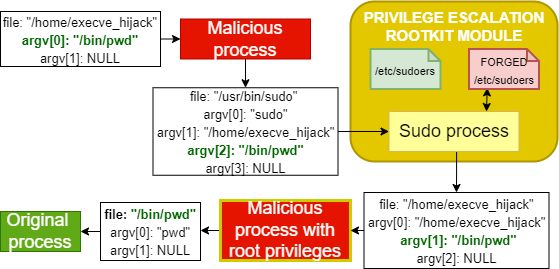
\includegraphics[width=14cm]{execve_hijack_overall_malware.png}
	\caption{sys\_execve calls of a malicious program to execute original hijacked program.}
	\label{fig:execve_hijack_overall_malware}
\end{figure}

As we can observe in the figure, the malicious program will create multiple sys\_execve calls, each with a different set of arguments:
\begin{enumerate}
\item Firstly, the malicious program receives the arguments modified from eBPF, where the original filename has been hidden in argv[0].
\item In order to be executed as sudo, the program crafts a new sys\_execve call for running itself as sudo. For this, it creates a sudo process, which will inspect arguments argv[1] and onwards to construct its own privileged sys\_execve call once it checks the user has sudo permissions. 

Since our malicious program does not have sudo permissions, we make use of the privilege escalation module we explained in section \ref{subsection:privesc} in order to modify the contents of the \textit{/etc/sudoers} file and tricking the sudo process into considering we have sudo privilege. After this, the sudo process makes a sys\_execve call to the malicious process, which this time will be running with root permissions.

\item Once the malicious program is running with root privileges, it can perform different actions in the infected machine. In our rootkit, this program (which can be found in ), establishes a connection with the remote rootkit client using a raw sockets-based protocol (which will be explain in section \ref{TODO}).

Apart from this, the malicious program will now run the original program, by taking argv[1] as the filename and considering the rest of the argv[] array, starting at position 2, as the program arguments (argv[1], argv[2]...). With respect to argv[0], its original value is easily recovered from the original filename. 
%TODO link to program in repository
\end{enumerate}


\section{Backdoor and C2}
This section covers a comprehensive analysis of the design, implementation and functioning of the rootkit backdoor and its C2 capabilities. As we explained at the beginning of the chapter, the rootkit will be capable of controlling all incoming and outgoing network traffic, and we will weaponize this capability to build a remotely controllable system which executes orders from the rootkit client.

Apart from the XDP and TC eBPF programs which compound the core of the backdoor module, we had to design and implement a series of network protocols which enable to communicate through the network with the rootkit client. Also, we will take into account that a firewall, or an Intrusion Detection System (IDS) \cite{ips} may be scanning the traffic, searching for suspicious packet. Therefore, we will attempt to camouflage our traffic as common traffic generated by benign applications. 

Note that IDSs and firewalls are usually located outside of the host, in the middle point between the router which connects to the Internet and the host. Therefore, it is not enough that we hide our rootkit packets from the kernel using XDP as we explained in section \ref{section:abusing_networking}, but rather we must aim to design packets which are not suspicious to be malicious even from the perspective of software that sits in the middle of all of our transmissions through the network.

\subsection{Backdoor triggers} \label{subsection:triggers}
After a machine is infected by the rootkit, the rootkit client program will be used by the attacker to initiate a connection with the backdoor. However, first and foremost the backdoor needs to be able to detect whether a packet corresponds to common traffic generated by the host applications, or if it is coming from the rootkit client. This is because the attacker may be launching the rootkit client from any IP address, and listening at any port, so the backdoor must learn this parameters from the rootkit client, whose identity must be "authenticated" before establishing a connection with it. The first packet or group of packets whose purpose is to instruct the backdoor about who is the rootkit client and initiate a connection is known as a "trigger".

Although there exist a wide variety types of triggers, each type offers different advantages and drawbacks. In our rootkit, we have implemented multiple triggers with the purpose of discussing multiple authentication options, ranging from simple keywords inserted on packets, to complex packet streams that are based on triggers found in real-world rootkits.

Note that, as we introduced in section \ref{section:networking_fundamentals}, we will be exclusively working with TCP/IP packets, but an eBPF backdoor is capable of operating with any protocol of the network stack.

\textbf{Keyword-based triggers}\\
These triggers are one of the simplest but also the most easily detectable by any program inspecting the network traffic. This type of trigger consists of including a keyword (a simple string) inside the payload of the TCP packet. Figure \ref{fig:keyword_trigger} shows an example of a trigger of this kind.

\begin{figure}[htbp]
	\centering
	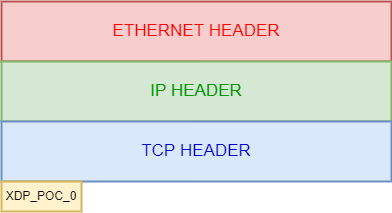
\includegraphics[width=10cm]{packet_examples_keyword_trigger.png}
	\caption{Keyword-based trigger on a TCP/IP packet.}
	\label{fig:keyword_trigger}
\end{figure}

Our rootkit is prepared to listen for keyword-based triggers, although it is a simple Proof of Concept (PoC) which does not take part in the main C2 functionality. In the case of the trigger shown in figure \ref{fig:keyword_trigger}, the rootkit will analyze the packet and detect that the pre-defined keyword "XDP\_PoC\_0" has been inserted into the payload, thus learning that the packet has been sent by the attacker. In the PoC implemented in our rootkit, this triggers an overwrite action, in which the XDP program will proceed to modify the payload and the packet size, changing the contents of the packet. This PoC can be seen in action in section \ref{TODO}.

\textbf{Port-knocking triggers}\\
This type of triggers is based on a common previously agreed sequence of ports which both the backdoor and the client share beforehand. When the client wants to initiate a connection with the backdoor, it will send an ordered sequence of packets directed to multiple of the ports of the infected host, so that the order of these ports corresponds to the sequence agreed with the backdoor \cite{port_knocking}. A backdoor sniffing network traffic will detect this pattern and initiate a connection with the source.

This type of trigger has not been implemented in our rootkit, although it has been discussed here for being one the most popular options.

\textbf{Advanced pattern-based triggers}\\
One of the main issues with keyword-based triggers is that, upon inspection of the packet, the trigger is easily reconizable (the payload contains a plaintext string) and this can lead to firewalls and IDSs flagging it as suspicious. 

We can, however, work on top of the idea of building a pattern that can be recognized by the backdoor, but at the same time seems random enough for an external network supervisor. This is the basis of some of the triggers we can find in real-world rootkit, such is the case of the rootkit Bvp47 \cite{bvp47_report}. %TODO the link is too slow, should we put our repository as a source?

Bvp47 is a rootkit with C2 capabilities built as a Linux kernel module developed by the NSA Equation Group and discovered by the research laboratory Pangu Lab \cite{pangu_lab}. One of its capabilities is communicating with a backdoor via pattern-based triggers. These triggers are seemingly random, but they follow a hidden pattern that only the entity who knows it will be able to detect it, acting as a "key". The triggers used in the Bvp47 rootkit consist of a TCP packet whose payload has been filled with random memory, with the exeception of a selection of bits which are the result of certain XOR operations \cite{bvp47_report_p49}.

The backdoor of our rootkit is capable of working with pattern-based triggers similar to those presented in Bvp47. Figure \ref{fig:bvp47_trigger} shows the trigger we implemented for our backdoor.

\begin{figure}[htbp]
	\centering
	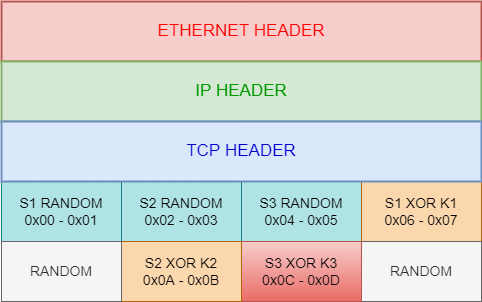
\includegraphics[width=10cm]{packet_examples_bvp47_trigger.png}
	\caption{Pattern-based backdoor trigger in our rootkit.}
	\label{fig:bvp47_trigger}
\end{figure}

As we can observe in the figure, a series of 8 data sections of 2 bytes of length each are included in the payload. Some of these are completely random, while others are the result of calculating operations involving other sections and some "keys". These keys are data shared by the backdoor and the rootkit client, and enable to encode hidden information in what would seem random data after they are XORed with other data. Specifically, the key K3 encodes the command which the rootkit client wants the backdoor to execute. Table \ref{table:k3_values} shows the values and the actions triggered by K3 once they are parsed by the backdoor. Table \ref{table:k1_k2_values} shows the shared values of K1 and K2, which do not trigger an action like K3, but serve to ensure that the value at the 7th data section (S3 XOR K3) was not generated by accident by another packet.

\begin{table}[htbp]
\begin{tabular}{|c|>{\centering\arraybackslash}p{8cm}|}
\hline
Value & Action\\
\hline
\hline
0x1F29 & Request to start an encrypted pseudo-shell connection.\\
\hline
0x4E14 & Request to start a 'phantom shell' connection (this is explained in section \ref{TODO}).\\
\hline
0x1D25 & Request to load and attach all rootkit eBPF programs.\\
\hline
0x1D24 & Request to detach all rootkit eBPF programs.\\
\hline
\end{tabular}
\caption{Rootkit actions related to K3 values in the pattern-based backdoor trigger.}
\label{table:k3_values}
\end{table}

\begin{table}[htbp]
\begin{tabular}{|c|c|}
\hline
Key & Value\\
\hline
\hline
K1 & 0x56A4\\
\hline
K2 & 0x7813\\
\hline
\end{tabular}
\caption{K1 and K2 values in the pattern-based backdoor trigger.}
\label{table:k1_k2_values}
\end{table}

The above format guarantees that two packets will never contain the same data, while at the same time the result is a TCP packet with random data. Therefore, when the backdoor receives any TCP packet, it will attempt to use K1, K2 and K3 to calculate the operations shown in figure \ref{fig:bvp47_trigger}. If the format matches, then it will instruct the rootkit module responsible to execute the action related to K3.

Although this type of trigger is stealthier than the previous we presented, its main drawback is that, upon a forensic investigation and decompilation of the rootkit and backdoor, the value of the keys can be found and therefore its traffic detected. 

Also, we want our TCP packet to be as similar to normal traffic as possible, therefore sending a single TCP packet without a previous 3-way handhsake would be slightly suspicious from a firewall standpoint. This is why the pattern-based trigger we have presented will be a SYN packet (in the TCP header, we set to 1 the SYN FLAG), so that the trigger could be seen as a normal request for initiating a connection.

Although using SYN packets is stealthier than sending single data packet without being in the context of a connection, it can be argued that SYN packets in a 3-way handshake do not usually have a payload. However, the TCP standard allows for the inclusion of data in SYN packets, and there exist some cases in which SYN packets with data are being actively used, such is the case of TCP Fast Open \cite{tcp_syn_payload} \cite{rfc_tcp4}. Also, we can find that firewalls such as Cisco do not drop SYN packets even if they have data by default \cite{cisco_syn_firewall}.


\textbf{Multi-packet stealthy triggers}\\
The final type of trigger incorporated into our backdooring system consists of a trigger composed of a stream of TCP packets with an empty payload field. In this case, the authentication of the rootkit client by the backdoor is achieved by hiding data inside some of the fields at the TCP or IP headers. 

This trigger is based on the one included on the implant called "Hive", from which various classified documents related with its development were leaked by WikiLeaks \cite{hive_implant}. In this implant, the developers designed a large data payload to send with their own implant remote controller, which was later divided into smaller chunks, each part being injected into a different TCP, UDP or ICMP packet in a packet stream. When the implant received these packets, it would reconstruct the original data by taking the payload from the received packets and joining the chunks in order of packet arrival.

In our rootkit, we will follow a similar approach, hiding a large set of data not in the payload of a TCP packet, but in the TCP headers itself. Our packets will also be marked with the SYN flag. By taking these two measures, the stream of packets would seem a harmless succession of SYN packets requesting to start a connection.

Firstly, the rootkit client will define the data payload to send as shown in figure \ref{fig:hive_data}.

\begin{figure}[htbp]
	\centering
	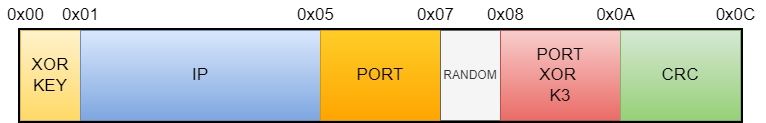
\includegraphics[width=13cm]{packet_examples_hive_data.png}
	\caption{Data payload sent by rootkit client using multi-packet trigger.}
	\label{fig:hive_data}
\end{figure}

As we can observe in the figure, the rootkit will tell the backdoor information about to which IP address the rootkit has to send back a response. This enables to send the multi-packet trigger from an spoofed IP address and port. It also contain another K3 XORed with the port, so that the backdoor knows which action is requested by the rootkit client. The values for this K3 are the same as we showed in table \ref{table:k3_values}.

The payload also contains two particularly relevant fields, a CRC and a XOR key:
\begin{itemize}
\item The XOR key will be used to calculate a rolling XOR over the whole payload before it is sent. This operation consists of calculating the XOR of each byte X with its adjacent X+1, and storing the result of the operation in byte X+1. Therefore, byte 0x00 is XORed with 0x01 and stored into 0x01, byte 0x01 XOR 0x02 is stored in 0x02, and we repeat the operation with the whole payload. The result is an seamingly random array of bytes, which may go under the radar of any software supervising the network.
\item The Cyclic Redundancy Check (CRC) is an error-detecting code commonly used to check for errors during data transmission \cite{crc}. By calculating the CRC of our payload we aim to ensure that the complete payload has been reconstructed successfully after transmitting it to the backdoor.

A CRC is necessary because we may receive corrupted packets (TCP guarantees integrity of data during a connection between applications, but we are capturing the packets from the kernel in the backdoor) and because a firewall may modify our packets before they reach the kernel at the host.
\end{itemize}

After the rootkit client has built the data payload to send, it will divide it into multiple chunks and inject them into some of the fields at the TCP headers. We have implemented two different triggers according to this:
\begin{enumerate}
\item The first type of trigger consists of dividing the payload into 3 chunks of 4 bytes each, and injecting them into the sequence number of SYN TCP packets, as shown in figure \ref{fig:hive_seqnum}.

\begin{figure}[htbp]
	\centering
	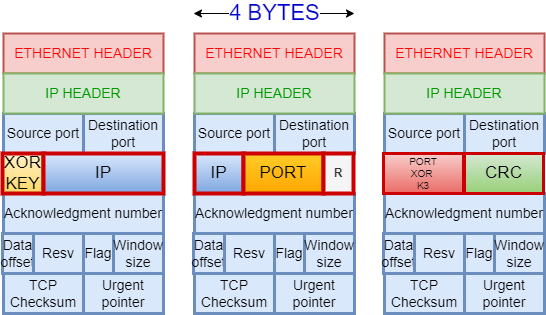
\includegraphics[width=14cm]{packet_examples_hive_seqnum.png}
	\caption{Multi-packet trigger with payload embedded in TCP sequence number.}
	\label{fig:hive_seqnum}
\end{figure}

\item The second type of trigger consits of dividing the payload into 6 chunks of 2 bytes each, and injecting them into the source port of SYN TCP packets, as shown in figure \ref{fig:hive_srcport}.

\begin{figure}[htbp]
	\centering
	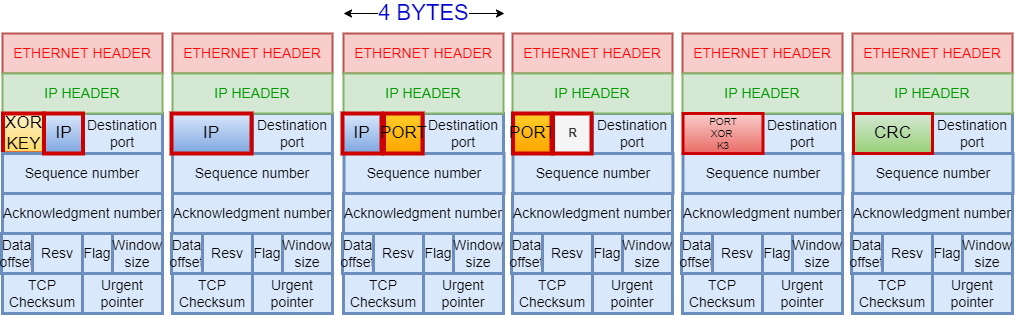
\includegraphics[width=14cm]{packet_examples_hive_srcport.png}
	\caption{Multi-packet trigger with payload embedded in TCP source port.}
	\label{fig:hive_srcport}
\end{figure}

\end{enumerate}

Note that, although in figure \ref{fig:hive_seqnum} and \ref{fig:hive_srcport} the data is injected directly, this data has been transformed under the rolling XOR, so a firewall or IDS would not easily reconstruct the IP or the PORT just by looking at the packet.

After the rootkic client constructs the packet stream to send, the packets are sent in order to the infected system and the backdoor will have to process them. The backdoor will only be able to acknowledge that a trigger has been sent after the 3 (or the 6) packets have been received, therefore the XDP program is in charge of saving the last 3 (or the last 6) packets received from each IP address at a minimum.

In our rootkit, this is achieved by using eBPF maps which work as a First-In-First-Out (FIFO) structure:
\begin{itemize}
\item The map backdoor\_packet\_log\_16 keeps a log of the last 3 packets received by each IP address, where the IP address is the key of the map.
\item The map backdoor\_packet\_log\_32 keeps a log of the last 6 packets received by each IP address, where the IP address is the key of the map.
\end{itemize}

By using the previous maps, the XDP program will first wait until 3 (or 6) packets are received, and afterwards attempt to extract the original payload for each new packet that arrives. For this, the XDP program will:
\begin{enumerate}
\item Extract the sequence number (or source port) from each of the packets in the map and concatenate the bytes.
\item Undo the rolling XOR operation.
\item Check that the CRC is correct.
\item Check that the field PORT XOR K3 is correct by trying with all the available values of K3, calculating (PORT XOR K3) XOR K3 and checking if the result is PORT.
\end{enumerate}

If the previous checks do not fail, it means the packet stream was a multi-stream trigger and the XDP program proceeds to execute the action corresponding to K3.



%TODO INTRODUCE IMAGES OF SHELLS
\subsection{Command and Control} \label{subsection:c2}
This section details the C2 capabilities incorporated in our rootkit, that is, mechanisms that enable the attacker to introduce rootkit commands (not to be confused with Linux commands in a shell) from the remote rootkit client and to be executed in the infected machine, returning the output of the command (if any) back to the client. These rootkit commands can be instructed by sending a backdoor trigger, which as we mentioned, depending on the value of K3 in the trigger, a different rootkit action will be executed by the backdoor (available values are displayed in table \ref{table:k3_values}).

Some of the actions triggered by the backdoor involve modifying the behaviour of the rootkit (such as attaching/detaching eBPF programs reotely), while others enable the attacker to spawn rootkit 'pseudo-shells'. These pseudo-shells are a special rootkit-to-´rootkit client connections which simulate a shell program, enabling the attacker to execute Linux commands remotely and get the results as if it was executing them directly in the infected machine. During this connection, the rootkit and the rootkit client will exchange messages containing commands and information. For this, both programs need to agree on a common protocol which is mutually understood, defining the format and content of these transmissions.

Apart from being able to spawn pseudo-shells by sending such action requests to the backdoor using a backdoor trigger, some other shells can also be spawned as a result of a successful exploitation of either the library injection module or the execution hijacking module. In particular, the malicious library we injected in section \ref{section:lib_injection} and the malicious user program of section \ref{section:execution_hijack} spawn one of these shells once they are executed.

As a summary, figure \ref{fig:c2_summ} shows an overview of C2 infraestructure.

\begin{figure}[htbp]
	\centering
	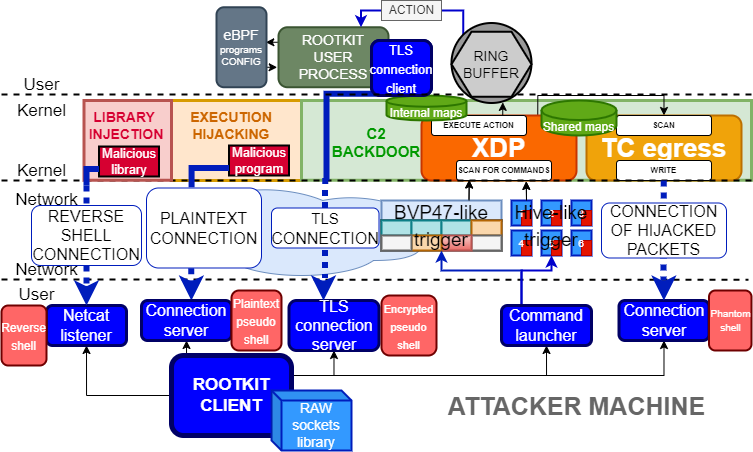
\includegraphics[width=14cm]{c2_summ_infra.png}
	\caption{Command and Control infraestructure of the rootkit.}
	\label{fig:c2_summ_infra}
\end{figure}

As we can observe in the figure, the rootkit client offers a command launcher, which sends backdoor triggers to the backdoor. The backdoor scans the traffic and executes the according action corresponding to K3. After that, the backdoor can use the ring buffer to instruct the rootkit user process to launch actions from the user space. One of this actions is starting an encrypted pseudo-shell connection, enabling the rootkit client to remotely execute commands in the infected machine. As we mentioned, other types of shells can be spawned, including a simple reverse shell by the malicious library of the library injection module, a plaintext pseudo-shell connection by the execution hijacking module, and a pseudo-shell based on packets hijacked by the backdoor called the 'phantom shell'. 

We will now proceed to analyse each of these connections and shell-like mechanisms which compound the C2 functionality.


\textbf{Reverse shell}\\
This is the simplest and most automated shell we can obtain from an infected machine. This shell is spawned when we inject the malicious library of the library injection module (section \ref{section:lib_injection}), therefore the parties involved in the transmission are the rootkit client and the malicious library.

A reverse shell is initiated from the infected machine to the attacker, that is, the malicious library actively initiates the connection, and the rootkit client must listen for this request using a netcat listener (or a similar program). A reverse shell is usually created in three steps:
\begin{enumerate}
\item Open a socket and setting a TCP connection with the attacker IP and listening port (other protocols may be used too).
\item Readjusting the three standard POSIX file descriptors in the infected machine (stdin, stdout, stderr) \cite{file_descriptors} so that they refer to the same file descriptor of the socket.
\item Executing a shell program (bash, sh).
\end{enumerate}

With the above setup, any command received in the socket (which is now a duplicate of file descriptor stdin) will be used by the shell program as an input. The shell program will execute the command and return the output in stdout, which since it is now a duplicate of the socket, it will be written into the socket, sending the message to the attacker through the network.

The attacker, for its part, can accept the TCP connection requested by the infected machine, opening a socket and writing to it to send commands, and reading from the socket to receive the output of the commands' execution on the victim.
 
 
 
\textbf{Plaintext pseudo-shell}\\
This shell-like connection enables the attacker to send commands, execute them in the infected machine and receive back the output without the execution of any shell program, and with all transmissions being sent in plaintext over the network.

This type of shell is obtained by running the malicious program of the execution hijacking module of the rootkit. The rootkit currently does not incorporate a backdoor trigger that launches this module, but rather it is started automatically once the malicious program is executed (see table \ref{table:k3_values}, we have not included a K3 for running an unencrypted pseudo-shell).

While running a plaintext pseudo-shell, the rootkit client and the malicious program from the execution hijacking module (hereafter called the rootkit, since it is part of it) will make use of a master/slave protocol where the rootkit client acts as the master (sending commands) and the rootkit acts as the slave (it only sends data in response of a client message). On each transmission, the rootkit client will send a single TCP packet (without a preceeding 3-way handshake) in which the command is embedded as the payload. The rootkit will execute this command and answer back with the output in another single TCP packet.

Apart from the data being transmitted (the command and the output of that command), we will find a protocol header embedded in the packet payload too. This header will be positioned starting at the first byte of the packet payload, preceeding any other data, which is written in the next byte right after the header ends. Figure \ref{fig:ups_packet_struct} shows the overall structure of one of the TCP packets being used in the protocol. Table \ref{table:ups_headers} shows the different headers and their meaning in the protocol.

\begin{figure}[htbp]
	\centering
	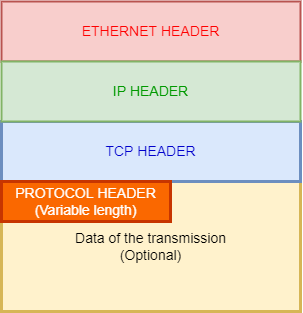
\includegraphics[width=7cm]{ups_packet_struct.png}
	\caption{Packet structure in a plaintext rootkit pseudo-shell.}
	\label{fig:ups_packet_struct}
\end{figure}

\begin{table}[htbp]
\begin{tabular}{|c|>{\centering\arraybackslash}p{8cm}|}
\hline
\textbf{Header} & \textbf{Description}\\
\hline
\hline
CC\_SYN & Sent by the rootkit client to the rootkit, requests to initiate a connection. Expects a packet with CC\_ACK in response.\\
\hline
CC\_ACK & Sent by the rootkit to the rootkit client, indicates readiness to initiate a connection.\\
\hline
CC\_MSG\# & Packet with data. If sent by the rootkit client, it contains a command. If sent by the rootkit, it contains the command execution output.\\
\hline
CC\_FIN & Sent by the rootkit client. Requests to terminate the pseudo-shell connection.\\
\hline
CC\_ERR & Sent by the rootkit. Indicates that the rootkit failed to parse the packet that the rootkit client sent.\\
\hline
\end{tabular}
\caption{Protocol headers in the plaintext rootkit pseudo-shell.}
\label{table:ups_headers}
\end{table}

Figure \ref{fig:ups_transmission} illustrates a common transmission following the described protocol.

\begin{figure}[htbp]
	\centering
	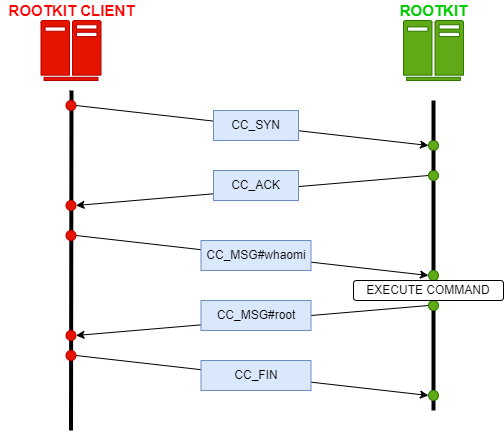
\includegraphics[width=11cm]{ups_transmission.png}
	\caption{Execution of a command using a plaintext rootkit pseudo-shell.}
	\label{fig:ups_transmission}
\end{figure}

As we can observe in figure \ref{fig:ups_transmission}, packets containing CC\_SYN and CC\_ACK act as a custom 2-way handshake. This step could be considered redundant and has been included only to share a resemblance with the TCP protocol.

Also, note that after a successful CC\_SYN-CC\_ACK exchange there is no need to repeat it after a CC\_MSG, the transmission will consist on consecutive CC\_MSG packets until the pseudo-shell is closed from the rootkit client with a CC\_FIN.


\textbf{Encrypted pseudo-shell}\\
Similarly to plaintext pseudo-shells, encrypted pseudo-shells enable the attacker to send commands, execute them in the infected machine and receive back the output, but all transmissions will be contained in the context of a secure encrypted connection using TLS.

In our rootkit, this type of shells are spawned after the rootkit client requests such an action to the network backdoor by setting the appropiate value of K3 (see table \ref{table:k3_values}) on either a pattern-based backdoor trigger or a multi-packet trigger. Once such a trigger is received in the backdoor, it will request to the rootkti user process to execute a TLS client that connects to the TLS server run at the rootkit client. 

Once both parties are connected using TLS, they exchange data using a custom protocol, similar to the one used for plaintext pseudo-shells, but this time using TLS-contained messages. This message exchange works as master/slave protocol too, where the rootkit client will send a command to the rootkit, and the rootkit will execute the command and answer back with the output. Similarly to plaintext pseudo-shells, these messages are composed of a header and the data being transmitted. Table \ref{table:eps_headers} show the headers according to the protocol.

\begin{table}[htbp]
\begin{tabular}{|c|>{\centering\arraybackslash}p{8cm}|}
\hline
\textbf{Header} & \textbf{Description}\\
\hline
\hline
CC\_COMM\_RQ\# & Sent by the rootkit client to the rootkit, sends a command to be executed.\\
\hline
CC\_COMM\_RS\# & Sent by the rootkit to the rootkit client, sends the result of an executed command.\\
\hline
CC\_FIN & Sent by the rootkit client. Requests to terminate the pseudo-shell connection.\\
\hline
CC\_ERR & Sent by the rootkit. Indicates that the rootkit failed to parse the message that the rootkit client sent.\\
\hline
\end{tabular}
\caption{Protocol headers in the encrypted rootkit pseudo-shell.}
\label{table:eps_headers}
\end{table}

As we can observe, this protocol works similarly to the one in pseudo-shells, with the only absence of the CC\_SYN and CC\_ACK messages. The reason for this is that, since the messages are contained in the context of a TLS connection, accepting the connection is considered as assurance enough that both parties are already synchronized.



\textbf{Phantom shell}\\
This shell-like connection works with the coordination of both the XDP and TC modules at the backdoor. It does not involve sending any packets from the user space, but rather the backdoor will reuse packets being sent by other applications in the infected machine, modifying them so that they are directed to the rootkit client. Afterwards, the original packet will be transmitted without modifications to its original destinatary due to the TCP retransmissions. This technique has been explained in detail in section \ref{subsection:network_attacks}.

A phantom shell can be obtained from the rootkit client by sending a backdoor trigger (only pattern-based triggers are supported for this shell) with the corresponding value of K3 (see table \ref{table:k3_values}). The XDP program at the backdoor receives the trigger and communicates to the TC program that the backdoor has been instructed to start a phantom shell. TC will modify a single packet and send it to the rootkit client, indicating that the backdoor is ready to start the phantom shell. After that, the client and the backdoor exchange TCP packets using a shared protocol (similar to that of plaintext pseudo-shells) in the following manner:
\begin{enumerate}
\item The rootkit client sends a TCP packet with the command to execute.
\item The XDP program at the backdoor scans the traffic and detects that a TCP packet belonging to a phantom shell has been received (recognizing it by its header at the TCP payload).
\item The XDP program tells the rootkit user space process to execute the command and obtain the output.
\item The rootkit user space program communicates the TC program the output of the command.
\item The TC program overwrite a packet and redirects it to the rootkit client.
\end{enumerate}

Both XDP and the user space rootkit program will communicate with the TC program using a shared map called backdoor\_phantom\_shell. This map only stores one single entry at a time, containing the following data:
\begin{itemize}
\item IP address indicated in the backdoor trigger to which the backdoor must write back to.
\item Port indicated in the backdoor trigger.
\item The command requested by the rootkit client (this is empty when XDP communicates having received the backdoor trigger in the first step).
\end{itemize}

With respect to the protocol being used, the TCP packets exchanged between the rootkit client and the TC program is the same as that shown in figure \ref{fig:ups_packet_struct}. The only difference is in the headers being used, which are described in table \ref{table:phantom_headers}.

\begin{table}[htbp]
\begin{tabular}{|c|>{\centering\arraybackslash}p{8cm}|}
\hline
\textbf{Header} & \textbf{Description}\\
\hline
\hline
CC\_PHANTOM\_INIT & Sent by the TC program to the rootkit client after receiving the pattern-based backdoor trigger indicating request to initiate a phantom shell.\\
\hline
CC\_PHAN\_RQ\# & Sent by the rootkit client to the backdoor, sends a command to be executed.\\
\hline
CC\_PHAN\_RS\# & Sent by the backdoor to the rootkit client, sends the result of an executed command.\\
\hline
CC\_ERR & Sent by the backdoor. Indicates that the rootkit user space program failed to parse the command that the rootkit client sent.\\
\hline
\end{tabular}
\caption{Protocol headers in the phantom shell.}
\label{table:phantom_headers}
\end{table}

As we can appreciate in the table, in contrast to the other pseudo-shells we have presented, there are not any headers indicating to close the phantom shell in this protocol. This is because there is no program listening to the messages such as in the previous cases (the encrypted pseudo shell used a TLS client, the other where run from the malicious library and malicious program from rootkit modules). In this case, however, the backdoor listens for each message and executes the commands individually, as in a stateless protocol (although it requires the starting backdoor trigger to authentica the rootkit client).

Figure \ref{fig:c2_summ_example} illustrates this expalantion by showing how the rootkit client executes a command using a phantom shell.

\begin{figure}[htbp]
	\centering
	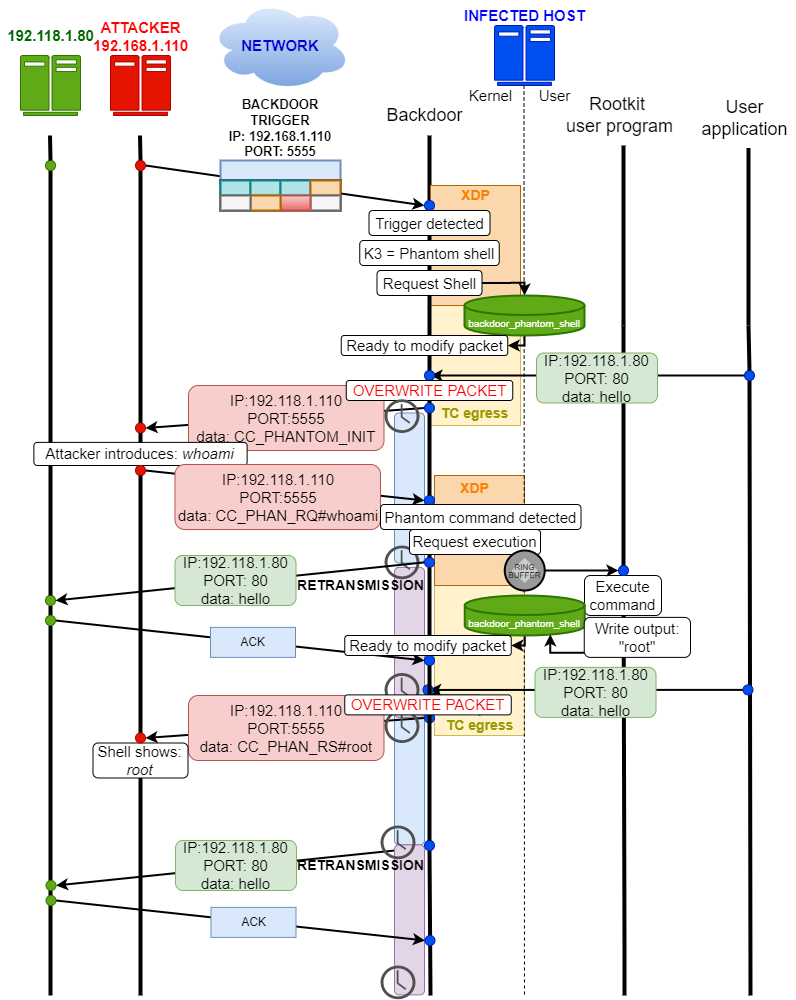
\includegraphics[width=15.5cm]{c2_summ_example.png}
	\caption{Execution of a command using the phantom shell.}
	\label{fig:c2_summ_example}
\end{figure}

As we can observe in the figure, the XDP program at the backdoor is responsible of sniffing the network for a backdoor trigger to authenticate an attacker and start the phantom shell or, afterwards, a phantom shell header. Once the XDP program or the rootkt user program write into the shared eBPF map that a phantom shell packet is needed to be sent, the TC egress program hijacks the first TCP packet that an user application requests to send through the network. TCP retransmissions ensure that this packet is eventually delivered.


\textbf{Backdoor commands}\\
Apart from supporting the remote execution of commands via the shell-like connections we have covered in this section, the backdoor also enables two other backdoor commands which modify the behaviour of the rootkit. As we can observe in table \ref{table:k3_values}, these commands consist on enabling or disabling eBPF programs remotely.

These commands are launched from the rootkit client, and get sent to the backdoor in the form of either a pattern-based trigger or any of the two forms of multi-packet trigger. As with any other backdoor trigger, the XDP program checks the value of K3 contained in the trigger and issues the corresponding action.

In the case of these commands, the order needs to be transmitted to the rootkit user space program, from where the eBPF programs will be attached or detached using the eBPF program configurator. We will cover the eBPF program configurator extensively in section \ref{TODO}.


\subsection{Backdoor internals}
This section offers insight into the functioning of the XDP and TC programs composing our backdoor. In particular, we will analyse their life cycle and operation, starting from the point when they are loaded and attached, and describing how they interact with the network traffic at the infected machine.

\textbf{XDP}\\
The XDP program is responsible of sniffing incoming network traffic and detecting backdoor triggers sent by the rootkit client. For this, it acts as a filter, where packets get passed to the kernel or go to the next filter depending on whether they meet certain criteria. Figure \ref{fig:c2_summ_xdp} illustrates the complete life cycle of the XDP program.

\begin{figure}[htbp]
	\centering
	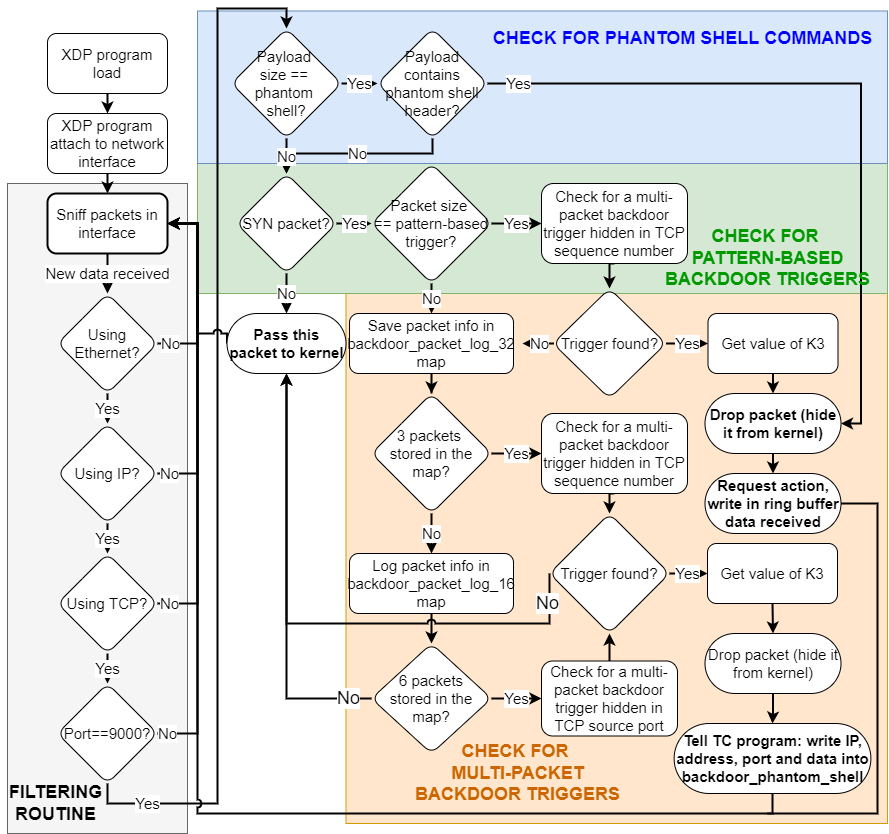
\includegraphics[width=15cm]{c2_summ_xdp.png}
	\caption{Life cycle of the backdoor XDP program.}
	\label{fig:c2_summ_xdp}
\end{figure}

As we can observe in the figure, the XDP program must be attached to a network interface of the infected machine (eth0, wlan0...). Once attached, it will repeatedly sniff the incoming network traffic.

For any packet received, a filtering routine will be applied, whose purpose is to discard any packet the backdoor will not work with, only keeping TCP/IP packets. Moreover, these initial checks done with the purpose of determining the protocol must always been made, otherwise the eBPF verifier may consider any access to the packet as invalid (since it will not be sure about the type and bounds of the fields it is accessing). We can also appreciate that the XDP program filters according to the destination port. The reason is that we have designed our backdoor trigger so that they are always directed to this port number.

After the initial filtering routine, the XDP program will check for any of the triggers or headers it could be receive to support the C2 capabilities of the backdoor. For this, more filters will be implemented, usually checking for the payload or packet size first, and later checking for the actual contentsm since the verifier forbids accessing payload data if its length is not assured. Also, in the case of working with multi-packet triggers, the related eBPF maps must be updated with the log of the latest packets received, as we described in section \ref{subsection:triggers}.

Once the type of trigger is detected, XDP proceeds to perfom the actions related to the value of K3 found inside each trigger. As we described in section \ref{subsection:c2}, these include writing into the ring buffer or communicating with the TC program via the shared eBPF map.

Note that in this diagram it has been omitted the section related with modifying incoming packets, used for the PoC shown in section \ref{TODO}. The reason is that its functionality is identical to that being shown in figure \ref{fig:c2_summ_tc} implemented by the TC program.


\textbf{TC}\\
The TC egress program is responsible for sniffing outgoing network traffic and modifying those packets needed for the C2 functionality, like the phantom shell. Similarly to the XDP program, it is composed of multiple layers of filters, whose purpose is to determine the packet protocol and the correctness of the data. Figure \ref{fig:c2_summ_tc} shows the complete life cycle of the TC program.

\begin{figure}[htbp]
	\centering
	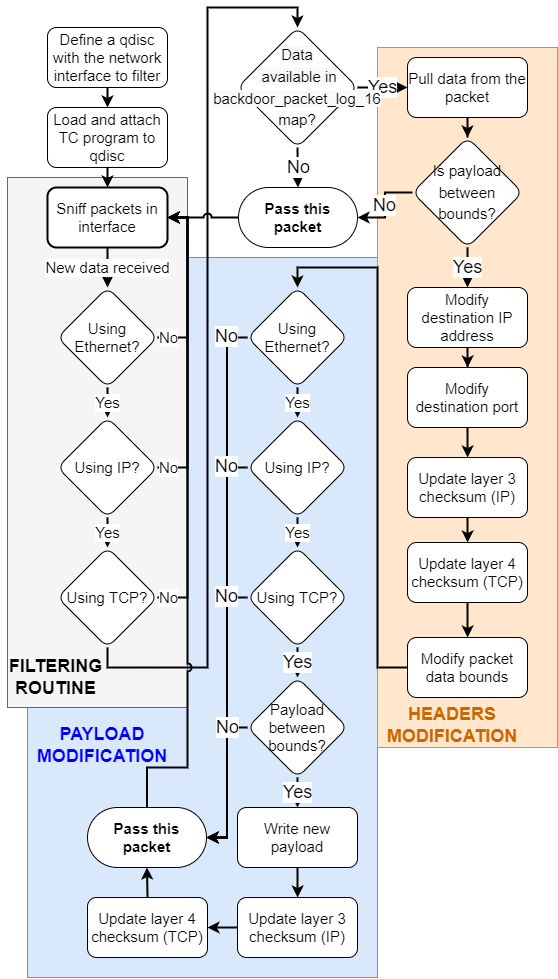
\includegraphics[width=13cm]{c2_summ_tc.png}
	\caption{Life cycle of the backdoor TC program.}
	\label{fig:c2_summ_tc}
\end{figure}

As we can observe in the figure, the TC program will ignore any packet until some data arrives at the shared eBPF map. At that point, it will proceed to overwrite the packet with the data it has been sent by the XDP or rootkit user process. In particular, it must redirect the destinatary of the original packet (thus changing the IP address and destination port) and modify the payload of the packet. Therefore, it approaches the packet modification in two steps:
\begin{itemize}
\item Modifying the IP and TCP headers of the packet with the new destination data.
\item Modifying the payload. Most of the times, this payload will be of different length compared to that of the original TCP packet, and therefore the TC program must modify the packet bounds. This is done using the bpf\_skb\_change\_tail helper, which we covered in section \ref{subsection:tc}. Note that, once we modify the packet bounds, the eBPF verifier will no longer trust our original checks with respect to the packet protocol and the validity of the payload. Therefore, all checks must be repeated before being able to overwrite the payload of the packet.
\end{itemize}

After the requested modifications are made, the TC program passes the packet to the next layer in the kernel.



\section{Rootkit client}
The rootkit client is a CLI program which the attacker can use from its own machine to communicate with the rootkit remotely over the network and execute commands using the C2 infraestructure. This section details its functionality and presents how it can be used to connect to the rootkit.

\subsection{Client manual}
The rootkit client is compiled to a single executable named \textit{injector}. This file must be run indicating which operation the attacker wants to issue to the attacker. Figure \ref{fig:client_help} shows the options which the client has available.

\begin{figure}[htbp]
	\centering
	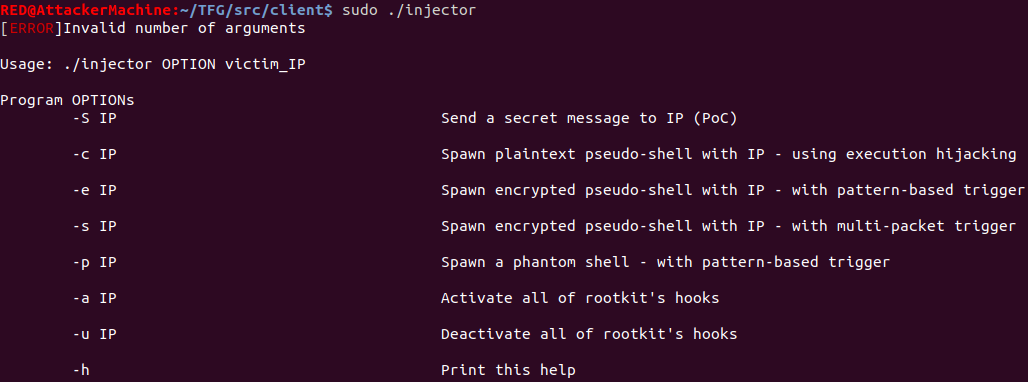
\includegraphics[width=15cm]{sch_client_help.png}
	\caption{Program options for rootkit client.}
	\label{fig:client_help}
\end{figure}

As we can observe in the figure, the rootkit client enables to execute the C2 actions we have described in section \ref{subsection:c2}. Upon running any of these options, the client will first request the network interface to use. This enables the attacker to choose the specific network to which it can connect to the infected machine.

After choosing an interface, the rootkit client crafts the respective backdoor trigger and sends it to the infected machine (we have also included an additional non-C2 PoC showing how the rootkit modifies incoming packets). Every option requires to specify the infected machine location by indicating its IP address.

After sending a backdoor trigger, the client will enter a listening state, waiting for the backdoor response. Once a response is received confirmating that the remote machine is up and the rootkit is installed, the client proceeds to show the user a shell prompt where it can enter commands. This shell prompt indicates whether we have spawned a plaintext, encrypted, or phantom psedo-shell. Figure \ref{fig:enc_shell} shows an encrypted pseudo-shell after receiving the backdoor response.

\begin{figure}[htbp]
	\centering
	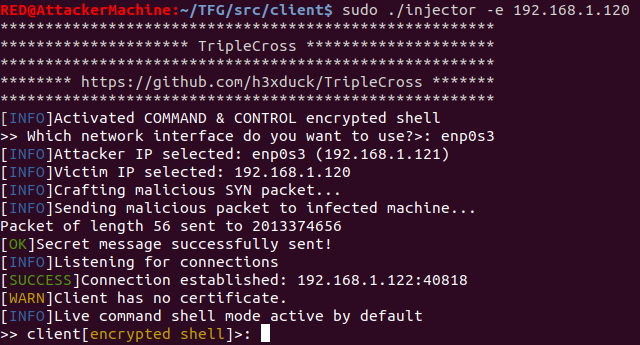
\includegraphics[width=15cm]{sch_enc_shell.png}
	\caption{Recently spawned encrypted pseudo-shell.}
	\label{fig:enc_shell}
\end{figure}

Once the command prompt appears, the attacker may introduce commands to be executed in the infected machine. Commands may only be introduced one at a time, since the client waits for the rootkit response before showing another command prompt. When the attacker finishes using the shell, it is recommended to close the connection gracefully. For this, the client supports "global commands", a special type of command which, when introduced in the shell, does not get sent to the rootkit but instead it triggers an action locally. Currently, although the infraestructure for supporting a large list of global commands has been developed, only one has been included. The attacker may introduce "EXIT" to close the connection gracefully (see in \ref{subsection:c2}, that packets for closing the connection are sent according to the protocol). Figure \ref{fig:enc_shell_comm_ex} shows the execution of multiple commands and closing the connection.

\begin{figure}[htbp]
	\centering
	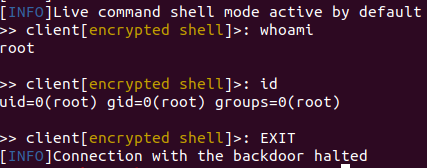
\includegraphics[width=12cm]{sch_enc_shell_comm_ex.png}
	\caption{Execution of commands with encrypted pseudo-shell and closing the connection.}
	\label{fig:enc_shell_comm_ex}
\end{figure}

As we can observe in figures \ref{fig:enc_shell} and \ref{fig:enc_shell_comm_ex}, the client also introduces multiple messages which provide additional information to the attacker about the state of the rootkit, the client and the ongoing connection. The existing message types are INFO, SUCCESS, WARN and ERROR.

Also, note that the rootkit client needs to be executed as root, since the library RawTCP\_Lib it uses requires privileges for some of its functionalities. 


\subsection{RawTCP\_Lib}
RawTCP\_Lib is the library on which the rootkit client delegates the task of building backdoor triggers, messages according to the rootkit protocol, and sending and receiving packets. This library is of our own authorship and available publicly \cite{rawtcp_lib}).

RawTCP\_Lib incorporates the following functionalities:
\begin{itemize}
\item Build and customize TCP/IP packets. This includes setting any arbitrary value on either the TCP or IP headers, enabling to customize every detail of the packet belonging to either the network or the transport layer (working with Ethernet headers is not supported).
\item Monitor the incoming network traffic, sniffing all received packets. Additionally, the library has support for sniffing packets with a certain data pattern in the payload.
\item Sending packets over raw sockets \cite{raw_sockets}, which enable us to send packets with our own custom headers.
\end{itemize}

Only by using RawTCP\_Lib, the rootkit client is be able to craft backdoor triggers whose data is contained in TCP headers (such as the multi-packet trigger). This gives us a great amount of freedom at the time of designing hidden messages. 

Apart from this, since raw sockets are indicated for reimplementing network protocols in the user space, it allows us to avoid undesired additional traffic in our rootkit transmissions. For instance, we do not need a 3-way handshake preceeding any of our transmissions.

Finally, the sniffing capabilities of this library are responsible of capturing the responses of the rootkit from the rootkit client. If we observe tables \ref{table:ups_headers}, \ref{table:eps_headers} and \ref{table:phantom_headers}, we can appreciate that the headers start at a common prefix "CC". This is used by the rootkit to sniff the network and capture any packet whose payload starts with that pattern.



\section{Rootkit user space program}
This section overviews the design and architecture of the user program that is launched with the rootkit. Its main responsability is loading and attaching the eBPF programs when the rootkit is executed, and of managing any further request of attaching or detaching programs during runtime that the backdoor may issue. Also, it interacts with the eBPF programs at the kernel in order to provide user space-only functionalities, such as executing commands. 

\subsection{Ring buffer communication}
The user space rootkit program communicates with the other components of the rootkit using two different means:
\begin{itemize}
\item A ring buffer, to which the program subscribes so that any new element written into it results in an event on the user program. Therefore it enables kernel to user space communication.
\item Other eBPF maps, on which the user program can write from the user space, thus enabling user to kernel communication.
\end{itemize}

In particular, the backdoor will be the responsible of most of the data written at the ring buffer, using it to request the actions corresponding to the commands received trhough the network (although the library injection module uses it too, see figure \ref{fig:flow_lib_injection_compact}. 

Any data written into the ring buffer is encapsulated in an "event", embodied by a struct \textit{rb\_event}. This struct supports all types data that any program using the ring buffer will need (thus not all of them are filled). In order to let the user program know which fields will need to be read for a given event, each \textit{rb\_event} is marked with an attribute \textit{event\_type}, which denotes the type of data that has been written in the buffer, and an attribute \textit{code}, that futher distinguishes events from the same type into their purpose. Table \ref{table:ring_buf_events} shows the event types and codes recognized by the user program:

\begin{table}[htbp]
\begin{tabular}{|c|c|>{\centering\arraybackslash}p{8cm}|}
\hline
\textbf{Event type} & \textbf{Code} & \textbf{Action requested} \\
\hline
\hline
INFO (0) & Any & Informative message, not requesting an action.\\
\hline
DEBUG (1) & Any & Debug message. Event currently deactivated.\\
\hline
ERROR (2) & Any & Reports an error from the kernel space. Event currently deactivated.\\
\hline
EXIT (3) & Any & Requests to stop the rootkit completely. Event currently deactivated.\\
\hline
COMMAND (4) & 0 & Requests to initiate an encrypted pseudo-shell.\\
\hline
COMMAND (4) & 1 & Requests to activate all hooks in the rootkit.\\
\hline
COMMAND (4) & 2 & Requests to deactivate all hooks in the rootkit.\\
\hline
PSH\_UPDATE (5) & Any & New packet with a phantom protocol header was received.\\
\hline
\end{tabular}
\caption{Events and their classification in the ring buffer.}
\label{table:ring_buf_events}
\end{table}


\subsection{eBPF programs configuration}
During the development of the rootkit, it has been our priority to aim for the greatest modularity and extensibility in order to facilitate the development of new rootkit modules, whilst at the same time enabling the possibility of attaching or detaching eBPF programs at runtime. Because of this we can find that, internally, the user space program of the rootkit divides into different modules the available programs depending on the functionality they implement. Table \ref{table:modules_list} shows this classification.

\begin{table}[htbp]
\begin{tabular}{|c|>{\centering\arraybackslash}p{8cm}|}
\hline
\textbf{File} & \textbf{Module} \\
\hline
\hline
fs\_module & Contains programs related to reading and writing files, such as the privilege escalation module.\\
\hline
exec\_module & Contains programs related to the execution of user programs, such as from the execution hijacking module.\\
\hline
injection\_module & Contains programs with the implementation of techniques related to memory injection, including the two stack scanning techniques for library injection.\\
\hline
xdp\_module & Contains programs related to the backdoor functionality.\\
\hline
\end{tabular}
\caption{Classification of eBPF programs from the user space.}
\label{table:modules_list}
\end{table}

In order to load and attach eBPF programs with different parameters and 
to enable managing them at runtime, the user space program uses the eBPF program configurator. This configurator consists on two configuration structs and an API that allows for manipulating the eBPF programs state dynamically. Code snippets \ref{code:configurator_modules} and \ref{code_configurator_modules_attr} show these two structures.

\begin{lstlisting}[language=C, caption={Program configurator struct with list of modules.}, label={code:configurator_modules}]
module_config_t module_config = {
    .xdp_module = {
        .all = ON,
        .xdp_receive = OFF
    },
    .fs_module = {
        .all = ON,
        .tp_sys_enter_read = OFF,
        .tp_sys_exit_read = OFF,
        .tp_sys_enter_openat = OFF,
        .tp_sys_enter_getdents64 = OFF,
        .tp_sys_exit_getdents64 = OFF
    },
    .exec_module = {
        .all = ON,
        .tp_sys_enter_execve = OFF
    },
    .injection_module = {
        .all = ON,
        .sys_enter_timerfd_settime = OFF,
        .sys_exit_timerfd_settime = OFF
    }
};
\end{lstlisting}

\begin{lstlisting}[language=C, caption={Program configurator struct with attributes for each module.}, label={code:configurator_modules_attr}]
module_config_attr_t module_config_attr = {
    .skel = NULL,
    .xdp_module = {
        .ifindex = -1,
        .flags = -1
    },
    .fs_module = {},
    .exec_module = {},
    .injection_module = {}
};
\end{lstlisting}

As we can observe in the snippets, one struct enables to define whether a module as a whole will be loaded and attached (with the setting "all") while also allowing for only loading specific eBPF programs within that module. On the other hand, the second struct contains relavnt attributes which are needed during the attaching process of the eBPF program. For instance, we can see that the xdp\_module requires and ifindex, which corresponds to the network interface to which the XDP module must be attached. These settings are set at runtime, since its value depends on the options with which the attacker executes the rootkit.

The user space rootkit program can modify any of the struct values following a request from the kernel eBPF programs. After setting the new values, it uses the configurator API to reload all eBPF programs. Table \ref{table:configurator_api} shows the available functions of the program configurator.

\begin{table}[htbp]
\begin{tabular}{|c|>{\centering\arraybackslash}p{10cm}|}
\hline
\textbf{Function} & \textbf{Description} \\
\hline
\hline
unhook\_all\_modules() & Detaches all eBPF programs.\\
\hline
setup\_all\_modules() & Parses the configuration structs and attaches them eBPF programs according to the specified configuration.\\
\hline
\end{tabular}
\caption{API of the program configurator.}
\label{table:configurator_api}
\end{table}

Therefore, the user space rootkit program will need to follow the next steps for loading and attaching the rootkit eBPF programs:
\begin{itemize}
\item Set as 'ON' those modules or specific programs that want to be attached in the \textit{module\_config} struct.
\item Load the appropiate value into the configuration attributes at the struct \textit{module\_config\_attr}.
\item Run the unhook\_all\_modules() function if this is not the first time that the rootkit is attaching the eBPF programs (it is not needed the first time right after the rootkit is executed, since programs are not attached yet).
\item Run the setup\_all\_modules() function to parse the configuration set in the structs and load and attach the eBPF modules and programs appropiately.
\end{itemize}



